\documentclass[conference]{IEEEtran}
\IEEEoverridecommandlockouts
% The preceding line is only needed to identify funding in the first footnote. If that is unneeded, please comment it out.
\usepackage{cite}
\usepackage{amsmath,amssymb,amsfonts}
\usepackage{algorithmic}
\usepackage{graphicx}
% \usepackage{graphics}
% \usepackage{adjustbox}
\usepackage{textcomp}
%\usepackage{xcolor}
\usepackage{hyperref}
\usepackage[hang,flushmargin]{footmisc}
%\usepackage{minted}
%\usepackage{appendix}
\usepackage{siunitx}
\usepackage{tabularx}
\usepackage[table]{xcolor}
% \usepackage{colortbl}
% \usepackage{tablestyles}
% \usepackage{geometry}
\usepackage{booktabs, multirow}
\usepackage{dblfloatfix}
% \usepackage[tableposition=top]{caption}
% \setlength{\parskip}{0.1mm}
\usepackage{titlesec}
\usepackage{url}
\usepackage[linesnumbered,ruled,vlined]{algorithm2e}    % longend
\newcommand\mycommfont[1]{\footnotesize\ttfamily\textcolor{blue}{#1}}
\SetCommentSty{mycommfont}
\SetKwInput{KwInput}{Input}                % Set the Input
\SetKwInput{KwOutput}{Output}               % Set the Ouput
\SetKwBlock{doparallel}{do in parallel}{end}
\SetKwBlock{return}{return}

\def\BibTeX{{\rm B\kern-.05em{\sc i\kern-.025em b}\kern-.08em
    T\kern-.1667em\lower.7ex\hbox{E}\kern-.125emX}}

\begin{document}

\title{Data Opinion Propagation in Deep Neural Networks\\
% {\footnotesize \textsuperscript{*}Note: Sub-titles are not captured in Xplore and
% should not be used}
% \thanks{Identify applicable funding agency here. If none, delete this.}
}

%\author{\IEEEauthorblockN{Hamed Karimi, Reza Samavi}
%\IEEEauthorblockA{\textit{Department of Electrical, Computer, and Biomedical Engineering} \\
%\textit{Ryerson University}\\
%Toronto, ON, Canada \\
%\{hamed.karimi, samavi\}@ryerson.ca}
%}

\maketitle
% The page numbers:
\thispagestyle{plain}
\pagestyle{plain}

% \import{sections/...}{abs}
\begin{abstract}
%In deep neural networks, the outcome of the classification task is determined based on the highest predictive probability of the target labels. The outcome probabilities of unselected target labels are either dismissed or considered as the uncertainty associated with the prediction. In machine learning research, this associated uncertainty is sometimes used as the only indicator of the model trustworthiness. 

In this paper, we 
%argue that this uncertainty is not adequately expressive and interpretable for trust quantification and 
propose a method to incorporate the uncertainty associated with the input data of a deep neural network and propagate this uncertainty throughout the training phase using subjective logic.    
%into the  and propagate the into nd model parameters in the trustworthiness of the learning model. According to the impact of training data distributional properties on the model performance, 
We represent intrinsic statistical properties of input data as subjective opinions and through the propagation of input data opinions, we    
%and propagate  attributes to initialize the input data opinions to be propagated through a DNN using Subjective Logic as a tool, to 
quantify the total opinion of the learning model that works as a trust metric for the outcome of the DNN. In our experiments, we demonstrate that statistical belief and uncertainty associated with the input data can impact the overall trustworthiness of a DNN model. 
%We also provide an analytical tool to study the trade-offs between projected trust probability and overall model accuracy. 
We observe that belief and projected probability of the final opinion of the model is increasing while uncertainty is decreasing.  
\end{abstract}

\begin{IEEEkeywords}
Deep Neural Network; Subjective Logic; Opinions; Uncertainty; Trustworthiness; Machine Learning;
\end{IEEEkeywords}

  
% In deep neural networks, the outcome of the classification task is determined based on the highest predictive probability of the target labels. The outcome probabilities of unselected target labels are either dismissed or considered as the uncertainty associated with the prediction. In machine learning research, this associated uncertainty is sometimes used as the only indicator of the model trustworthiness. In this research, we argue that this uncertainty is not adequately expressive and interpretable for trust quantification and propose a novel approach to incorporate uncertainty associated with datapoints and model parameters in the trust metric of the learning model. We leverage Subjective Logic as a tool to propagate and measure the uncertainty in DNNs, with an aim of quantifying total uncertainty in a decentralized federated learning system. We specifically focus on the federated learning application domain as trust in this domain is a make or break factor in aggregated model outcome. We demonstrate that statistical uncertainty (e.g., based on explained variance or eigenvalues) associated with the datapoints and belief or disbelief on model parameters can impact the overall trustworthiness of an FL model. We also provide an analytical tool to study the trade-offs between projected trust probability and overall model accuracy. This approach is particularly helpful in FL context when a culprit node needs to be identified in an objective and timely manner. 


% %%%%%%%%%%%%%%%%%%%%%%%%%%%%%%%%%%%%%%%%%%%%%%%%%%%%%%%%%%

% One of the trust criteria which is not well addressed in deep neural networks is the amount of uncertainty. Uncertainty in ML applications is a first-order uncertainty (Aleatory, Epistemic, or the hybrid version) to quantify a degree of uncertainty which is not expressive and will be applied in some specific circumstances. To be more expressive, there is a need to a second-order uncertainty other than prior uncertainties, to be applied and fused in a higher level in terms of considering other properties. We leverage Subjective Logic as a tool and inject it to deep neural networks in order to propagate and measure the uncertainty in a single DNN, with an aim of propagating and quantifying total uncertainty in a decentralized federated learning system. Furthermore, using subjective logic in our proposed approach is fully beneficial and adequately flexible in different DNN architectures since it can act as an add-on in a ML system by being applied along with the training process in each DNN, therefore, it has no significant additional computational burden. It is also compatible with the state-of-the-art methods of communication amongst different DNNs. The objective of our research is to develop a novel method for propagating uncertainty associated with training dataset as subjective opinions through a DNN model leading to the total model opinion containing total model uncertainty. Thus, we exploit some statistical and conceptual method to quantify and initialize data uncertainty and opinions to be propagated based on the nature of input data features. During training process, the model updates its parameters' opinions and outputs its total opinion. Each feature or label opinion individually participates in training process. Therefore, for opinion propagation through a network, the opinions of data features and labels are separately initialized. 
% We evaluate our proposed method using two real-world datasets, SUSY and KDD CUP 99, containing numerical and categorical features which are considerably different in terms of many statistical, natural, inferential, and domain aspects. Based on our evaluation, we expect a DNN model with higher accuracy indicates lower uncertainty. Therefore, we observe that by decreasing loss and increasing accuracy during our training epochs which is the sign of successful learning, the amount of belief is increasing while our model uncertainty is decreasing significantly. We show that the belief and uncertainty will be improved in a DNN model based on its loss function optimization during training process. Moreover, we indicate the impact of successful training and loss optimization on the total opinion and its determinants in the learning model. We also demonstrate the impact of different statistical or conceptual factors of data opinion initialization over total model opinion’s determinants like belief and uncertainty in a way that each opinion determinant is relatively improved during training epochs. As a future work, we are currently working on propagating data and model opinions through a decentralized federated settings in which we can train different client models over their private data without sharing confidential data information to achieve an improved global model. We intend to quantify the total uncertainty of a federated network based on propagated clients’ opinions over a specific amount of training rounds. Therefore, we utilize our approach in each communication, aggregation, and propagation activities in federated learning without a significant computational cost.



\section{Introduction}
\label{intro}

AI technologies are contributing to a wide range of decision-making processes, from driving a car, cancer diagnosis~\cite{hope,sl} and even providing legal advice~\cite{deeplearning}. 
Although the level of autonomy for an AI-based solution might be different in each usage scenario, the trend is increasingly towards human-independent, algorithmic decision-making. 
%For example, in driver-less cars all decisions are made by AI and the algorithms take complete control of the cars, whereas in medical diagnosis and intervention or legal aid, the AI systems recommend the best course of action to a health practitioner or the legal team, respectively. In both cases, the human decision making processes are highly influenced by the automated decisions made by AI-based systems. 
Since machine learning (ML) algorithms are at the core of AI systems, in such scenarios, a significant challenge is answering the question of how much trust we can put into the outcome of the ML model. An important factor contributing to the trustworthiness of ML models is uncertainty associated with input data. This uncertainty can be originated from the intrinsic properties of available data (e.g., missing data, imbalanced data, skewness) or even a subjective opinion expressed by a modeler. In either case, the trust question can be answered only if the modeler is able to take into account the opinion about the data in the training phase of an ML model and report the outcome of the model not only in terms of the model performance but also, in terms of the trustworthiness of the model.

In this paper, we propose a method of quantifying and propagating input data opinions throughout the training phase of a deep neural network. As of the state-of-the-art opinion propagation model proposed in~\cite{hope}, we are also inspired by the probabilistic logic framework defined as Subjective Logic (SL)~\cite{sl}. We first investigate the limitation of the opinion quantification and propagation method proposed in~\cite{sl}. We introduce the concept of \emph{interpretable opinions} that allows to capture the intrinsic statistical properties of input data as opinion determinants. To initialize input data opinions, we partition input data into numerical and categorical features and use statistical properties such as skewness and kurtosis. Then we extended the propagation method to be aligned with the newly introduced interpretable opinions. Moreover, we identified a shortcoming in the current method when computing the error opinion, the difference between predicted and actual outcomes (the error) of the DNN model is compared with a single threshold to form the error opinion missing to take into account uncertain evidence about the error. 
%while the This comparison yields to identify positive or neg an  ative evidence to form an error opinion.By Using the interpretable opinions, we   
%of  darta  and then t_method that quantifies the trustworthiness and total model opinion of a DNN using subjective logic. 
%{\color{blue}Moreover, the current method compare the the difference of predicted and actual outcome of the DNN model with a single threshold. This comparison yields to identify positive or negative evidence to form an error opinion.} 
%Then, we address the limitations of the current method in Section~\ref{limit}. 
%In our proposal We overcome these limitations by proposing a new method to incorporate input data opinion originated in statistical intrinsic properties of input data in opinion propagation method. Input data features are partitioned into numerical and categorical features, and target labels to be initialized by different interpretable statistical factors. 
%Finally, we evaluate our proposed method to investigate the impact of statistical properties of input data on the trustworthiness and total opinion of the DNN model. 
The experimental evaluation of the proposed method demonstrates that during the training process, the trustworthiness of the model is improving while the uncertainty is decreasing according to the different data opinion initialization factors.

We are making the following contributions: 1) we demonstrate the limitations of the current trust quantification model, 
%investigate the impact of intrinsic properties of input data such as mini-batch data like skewness on the model performance to quantify training data opinions. 
2) we extend the state-of-the-art propagation model to take into account input data opinions determinants (i.e., belief, disbelief, and uncertainty) and also enhance the opinion optimization process by incorporating uncertain evidence, and 3) we conduct an extensive experiment using real-world datasets, to demonstrate the effectiveness of our approach.  

%demonstrate that the impact of intrinsic properties of input data on the model performance and then show the reliability of the measured trustworthiness of a DNN using our proposed method. 
%Second We incorporate these distributional metrics based on the distributions of mini-batches of training data.
%{\color{blue} We enhance the optimization process by considering uncertain evidence, i.e. not necessarily positive or negative evidence, in model predictive outputs.}







%\section{Data Opinion Propagation Model}
\section{Current Opinion Propagation Models}
\label{method}

The following section provides the necessary preliminaries on the background of uncertainty and subjective logic as an approach leveraged to propagate data opinions in a DNN. Then, we provide subjective logic concepts and a summary of the current method of opinion propagation proposed by~\cite{hope}. Finally, we propose our method for the data opinion initialization and optimization process.
 
\subsection{Preliminaries and Background}
\label{background}

% \subsection{Single Deep Neural Network}
% A Deep Neural Network (DNN) is a computational network that can be considered as a function $\mathcal{F}_\Theta:~\mathcal{D} \rightarrow \hat{Y}$ in which $\mathcal{D}$ is a set of input data fed into the network, $\Theta$ is a set of network parameters (weights and biases), and $\hat{Y}$ is the output set of the approximated values $\hat{y} \in \hat{Y}$. Moreover, the DNN model $\mathcal{M}_{\Theta}$ aims to be trained based on its input data (a finite set of training data) denoted by $\mathcal{D}$, according to the function~$\mathcal{Q}:~\mathcal{D}~\rightarrow~Y$ such that, 
% \[
% \mathcal{Q} = \{\ (d_{i},y_{i})\ |\ i \in \mathbb{N}^{[1,m]}\ \}\ ,
% \]
% where $i$ is a data point with $d_{i}$ and $y_{i}$ representing features and target (label), respectively and $m$ is the number of participating data points (data samples) in the training dataset.

% In the DNN model $\mathcal{M}_{\Theta}$, we intend to optimize a loss function in the form of $\mathcal{L}(\mathcal{D},\Theta;Y)$. This optimization is performed by minimizing the average of each data sample $i$'s loss value with respect to the parameter set of $\Theta$ defined as, 
% \begin{equation}
% \min_{\Theta}\ \mathcal{L}(\mathcal{D},\Theta;Y) = \frac{1}{m}\ \sum_{i=1}^{m} loss(d_{i},\Theta;y_{i})\ ,
% \label{loss}
% \end{equation}
% where $loss(d_{i},\Theta;y_{i})$ is the loss function of the single data sample $i$ in the training dataset.

%%%%%%%%%%%%%%%%%%%%%%%%%%%%%%%%%%%%%%%%

% In deep learning, the layers of a DNN are either inner (hidden) layers, logits, or softmax. The number of inner layers could be different from one DNN to another depending on the application, input data, number of data features. However, the latter two layers are common among all DNNs in classification tasks. The logit layer is the second last layer and provides a set of $\hat{y} \in \hat{Y}$ generated by the last hidden layer of the DNN model such that $|\hat{Y}|$ is the number of labels. The softmax layer is the last layer that normalizes the output of logit layer into the probability vector $P_{\hat{Y}}$ as the final output of $\mathcal{M}_{\Theta}$. Softmax function generates the set of probabilities $P_\hat{Y}$ associated with each logit $\hat{y}$ for each target label $y_{l}$. Each $p_{\hat{y}} \in P_{\hat{Y}}$ is the probability of the target label $l \in L$ being selected while classifying an input data $\mathcal{D}_i$ in $\mathcal{M}_{\Theta}$. Formally, in the softmax layer, each neuron $i$ corresponding to the label $l$, computes the probability $p_{\hat{y}}$ of the output probability vector $P_{\hat{Y}}$ as,
% \begin{equation}
%     P_{\hat{Y}}=softmax(\hat{Y})=\{\ \frac{e^{\hat{y}_{i}}}{\sum_{i=1}^{n_l} e^{\hat{y}_{i}}}\ \}_{i \in \mathbb{N}^{[1,|\hat{Y}|]}}\ ,
% \label{softmax}
% \end{equation}
 
% Accuracy as an important indicator of the model performance, is obtained based on the set of logits $\hat{Y}$ of the DNN model $\mathcal{M}_{\Theta}$.

%%%%%%%%%%% IMPORTANT %%%%%%%%%%%%%%%%%
% As it can be seen in the Fig.~\ref{dfl},
% \begin{figure}[H]
% 	\centering
% 	\includegraphics[scale=0.4]{figures/rp.png}
% 	\caption{An example of decentralized federated settings: The temporary head will be determined and selected to aggregate the updates of the participating models using local differential privacy in each training round $t$ in order to quantify Trust and uncertainty in this settings based on subjective logic.}
% 	\label{dfl}
% \end{figure}

%\vspace {.3cm}
\noindent
\textbf{Uncertainty.}
In the DNN classification task (see Appendix~\ref{dnn_app}), the outputs of the model are the softmax probabilities $p_{\hat{y}} \in P_{\hat{Y}}$, and are considered as the confidence of the DNN model in selecting the target labels for the training data $\mathcal{D}$~\cite{deeplearning,confidence}. 
% For example, in the task of classifying the data sample $\mathcal{D}_i$ into one of the three labels \textit{\{Airplane, Car, Truck\}} with $P_{\hat{Y}}=\{0.02,\ 0.8,\ 0.18\}$, the label $l=$ \textit{`Car'} will be selected for $\mathcal{D}_i$ with the highest confidence (probability) of 0.8. 
% However, there are informative confidence or probability values for other labels which indicates how much confidence the model $\mathcal{M}_{\Theta}$ has for each label regardless of $d_i$ being correctly classified or misclassified. 
%To address the first-order uncertainty,

The total uncertainty of a DNN model is generally defined as the lack of confidence in classifying each data sample $d \in \mathcal{D}$. This uncertainty denoted by $U_{d}$, is calculated using the entropy of the probability vector $P_{\hat{Y}}$ as,
\begin{equation}
U_{d}(P_{\hat{Y}}) = - \sum_{\hat{y} \in \hat{Y}} p_{\hat{y}}\log p_{\hat{y}}\ .
\label{entropy}
\end{equation}

There are two types of uncertainty that can be used in deep learning: first-order and second-order uncertainty. %Traditional probability (probabilistic logic) represents first-order probability that develops information about the statements and expresses the relationship between those statements. Each statement is a meaningful declarative sentence that is evaluated to be true or false. 
$U_{d}$ is a first-order type uncertainty, quantified by the first-order probability of softmax function~\cite{uncer4,uncer5}. 
However, first-order probabilistic logic is limited in capturing ownership of the assigned or computed probability. For example, the probability extracted from softmax function may change, when the modeler or any other sources in a DNN (e.g., a neuron) has a certain opinion about the model outcome probability (or model performance) generated by the softmax function. To capture this notion, second-order uncertainty is defined as the probability  %may be understood as the probability 
that the first-order uncertainty has a certain value. This value can be interpreted as the value that would be assigned if certain information about the first-order probability were available, including opinions of a modeler or any other sources. In addition, we may encounter situations where the owner or the source cannot produce probability for the first-order uncertainty or where multiple owners or sources have different opinions about the uncertainty. 




%has three main limitations 1) in capturing ownership of first-order probabilities. For example, first-order probabilities like softmax probability does not have any owner (or source) to hold and present the probability. 2) the situation when an owner cannot produce probability for a random variable is not considered (no uncertainty is considered) 3) the situation where multiple owners or sources have different opinions about a statement, is not captured.

%A second-order uncertainty captures the probability  
%may be understood as the probability 
%that the first order uncertainty has a certain value. This value can be interpreted as the value that would be assigned if certain information about the first order probability were available, including opinions of a modeler or any other sources. 



%quantifies the probability of random variables 
%containing individual statements

% {\color {red} RS: WHY only ? what is statement?}

%%%% important %%%%
% We can use averaging to calculate total training uncertainty and total training confidence in each target label $l$ over all training data. Moreover, the maximum uncertainty resulted from the entropy equation is gained by uniformly assigning probabilities over all the classes (target labels).
%%%%
% The aforementioned uncertainty is captured and decomposed to two different types in deep learning~\cite{uncer-rev}: \textit{Aleatoric Uncertainty} (or data uncertainty) and \textit{Epistemic Uncertainty} (or model uncertainty). Aleatoric uncertainty comes from the noise inherently exists in input data and associated with information loss in representing real-world data samples. Therefore, this uncertainty cannot be reduced by training over adequate amount of data or improving training procedure. Aleatoric uncertainty is further divided into two different sub-categories:
% \begin{enumerate}
%     \item \textit{Heteroscedastic uncertainty} (data-dependant)  which is dependent to the input data and is predicted as a model output.
%     \item \textit{Homoscedastic uncertainty} (task-dependant) which is not dependant to the input data and stays constant for all input data and differs among various tasks.
% \end{enumerate}
% }
% Epistemic uncertainty is the uncertainty rooted in the model parameters and caused by insufficient coverage of training data, errors in training process, errors caused by unknown data or errors in model architecture. Thus, epistemic uncertainty can be reduced by training the DNN over an adequate amount of data, improving model structure, or rectifying training process~\cite{uncer-rev}. 

% Probabilistic logic (traditional probability) indicates first-order uncertainty using first-order probability. First-order probability quantifies the probability of only random variables containing individual statements. 
% Both aleatory and epistemic uncertainty present first-order uncertainty~\cite{uncer-rev}. 
% For example, $x$ is an individual statement of a binary random variable $\mathbb{X}=\{x,\overline{x}\}$ like flipping an unfair coin. When $x=head$, the probability of obtaining $head$ in flipping this coin can be $P(x)=0.6$ which demonstrates an amount of uncertainty in obtaining the individual statement $x \in \mathbb{X}$.

%A second-order probability Q(P) may be understood as the probability that the true probability of something has the value P. “True” may be interpreted as the value that would be assigned if certain information were available, including information from reflection, calculation, other people, or ordinary evidenc


%First-order probabilistic logic has three main limitations in capturing uncertainity originated from the ownership of opinions ~\cite{sl}: 1) the amount of the analyst's confidence cannot be captured, 2) the situation when the analyst cannot produce probabilities for some input arguments, is not considered, and 3) the situation when multiple sources have various certain opinions (beliefs) about the same statement. Subjective logic as a tool prevents the above limitations to extend probabilistic logic using second-order logic considering uncertainty about probabilities as well as beliefs about a statement~\cite{sl}. More specifically, second-order probability computes the probability over functions or sets of individuals as well as the very individuals. Second-order uncertainty is represented in the form of the Beta or Dirichlet probability density functions (PDF) over first-order probabilities. 
% {\color{red}
% RS: HAS TO BE REWRITTEN- many problems: FIRST you should say there are other types of uncertainty, THEN you should define what is statement and their truth value. THEN you should say there are is second order... to capture these type of uncertainty, THEN define second o u} 
% We need to resolve the limitations of using probabilistic logic in order to be used in propagating the uncertainty in a DNN. 

\vspace {.3cm}
\noindent
\textbf{Subjective Logic}.
Subjective Logic extends probabilistic logic by including uncertainty about first-order probabilities and subjective belief ownership~\cite{sl}. Subjective logic utilizes arguments called \emph{Opinion} expressing separate beliefs about the truth of statements under an uncertainty mass as a second-order uncertainty. Although uncertainty generally means the lack of confidence, in subjective logic, uncertainty is the vacuity of evidence. This opinion representation is equivalent to the Dirichlet distribution and shows ownership of an opinion. 
Furthermore, subjective opinion ownership is closely related to trust since when there are different opinions about the same first-order probability, then a source can determine trust levels in other different sources of opinions before being integrated in a reasoning model~\cite{sl}.

% There are two main definitions we use in this research:

% \noindent\textbf{Definition 1:} A DNN Component $v$ is either an input data feature, a parameter (weight or bias), a neuron, or the entire neural network.{\color {red} RS: THE COMPONENTS ARe obviously not disjoint?!}
%DNN model 
%which containing data and participating in computational operations, 
%are considered as components of a neural network model. % $\hfill \blacksquare$

% {\color {red} RS: BIG GAP!! in introducing subjective logic concepts.  OPINION needs to be defined, then none of $b_v, d_v, u_v$ are defined.  the whole things also doesn't  belong here - perhaps should be part of your methodology  }

% {\color {red} RS: REWRITE - VERY POORLY WRITTEN \noindent\textbf{Definition 2:} Trustworthiness of a DNN component $v$ is defined as the projected probability of an opinion.  Since DNN components impact the model performance in each training epoch, following subjective logic, each DNN component $v$ has a binomial opinion $O_v=\{b_{v},d_{v},u_{v},a_{v}\}$ about the DNN model performance 
% %a subjective concept which is the model performance (accuracy) 
% such that $b_v + d_v + u_v = 1$. Moreover, the projected probability of an opinion $PP_v = b_v + u_v.a_v$ is considered as the trustworthiness of the component's opinion since it is an expected probability of all the opinion's determinants~\cite{sl} (see Appendix~\ref{sl_app} for more details).}  

\subsection {Current Method of Opinion Quantification}
\label{current_method}
We use the following definitions from subjective logic to capture second-order uncertainty to design our data opinion quantification model. 

% In the following, the required definitions and concepts in subjective logic are provided:
 
\vspace{.2cm}
\noindent\textbf{Definition 1 (DNN Component).} In a DNN, an input data feature, a model parameter (weight or bias), and/or a neuron are considered as DNN components.

\vspace{.2cm}
\noindent\textbf{Definition 2 (Binomial Opinion).} An opinion about a subjective variable $x$ in a binary domain $\mathbb{X}=\{x,\overline{x}\}$ is a \emph{Binomial Opinion} owned by a DNN component. A binomial opinion~\cite{sl} by the DNN component $v$ about the model performance as the subjective variable, is defined as a tuple of four determinants, % $\hfill \blacksquare$
\begin{equation}
    O_{v} = \{b_{v},d_{v},u_{v},a_{v}\} \quad \text{s.t.} \quad b_v,d_v,u_v,a_v \in \mathbb{R}^{[0, 1]}\ ,
\label{op}
\end{equation}
where $b_v$ denotes the amount of belief in support of the subjective variable $x$, $d_v$ denotes the amount of disbelief about $x$, the uncertainty mass $u_v$ represents the lack of confidence about $x$ caused by vacuity of evidence in a DNN model, and $a_v$ is the prior probability about $x$ without considering any evidence which can take a prior bias measure into account (see Appendix~\ref{sl_app} for more details on opinion determinants). 

Furthermore, these opinion masses should meet the following additivity requirement: 
\begin{equation}
b_v + d_v + u_v = 1\ .
\label{additivity}
\end{equation}

A binomial opinion by the DNN component $v$ is equivalent to a Beta PDF which is a particular binary version of Dirichlet PDF~\cite{sl}. The expected probability of the PDF yields to a projected probability as \emph{trustworthiness} of a DNN component which considers the component's belief and uncertainty about model performance simultaneously as,
% Therefore, a bijective mapping between a binomial opinion and a Beta PDF is defined as the equality between the expected probability of a Beta PDF and the projected probability of a binomial opinion~\cite{sl}. Therefore, this expectation can yield to a projected probability as trustworthiness of a DNN model which is considering the model belief and uncertainty about model performance simultaneously as, 
\begin{equation}
    \text{Projected Probability:} \quad PP_v = b_v + u_v.a_v\ .
\label{projprob}
\end{equation}

Since DNN components impact the model performance in each training epoch, following subjective logic, each DNN component $v$ has a binomial opinion about the DNN model performance. Furthermore, there are binary~\cite{sl} or multi-source operators~\cite{multi1} defined in subjective logic like Multiplication ($\otimes$), Comultiplication ($\widehat{\otimes}$), Average Fusion ($\oplus$), Cumulative Fusion ($\widehat{\oplus}$), and Multi-source Average Fusion ($\bigoplus$), to calculate the output opinion achieved based on a specific relation amongst two or more opinions as operands. 

Based on the the opinion propagation method in~\cite{hope}, for each feature of each data point $d \in \mathcal{D}$ such that $d=\{f_1,f_2,...,f_n\}$ with the true label $y \in Y$, the data feature opinions are initialized by given and equal opinions $O_d = \{O_{f_j}\ |\ j \in \mathbb{N}^{[1,n]}\}$ as feature opinion set and $O_y$ as true label opinion. These data opinions are propagated through the DNN similar to the data forward propagation. In each layer $i$, the forward propagation is fulfilled by the multiplication of the last layer neurons' opinions and the corresponding weight opinions denoted by $O_{w_i}$. For the first hidden layer, the multiplication is done between weight opinions and data opinions. {\color{blue} Thus, each neuron's opinion is dependent to the opinion of weights and the previous layer's neurons.} Then, in the layer $i$, the opinion of each neuron denoted by $O_{N_i}$, is achieved by combining these multiplications together along with the bias opinions denoted by $O_{b_i}$:
\begin{align}
O_{N_1} &= \bigoplus(O_{D} \otimes O_{w_1}, O_{b_1})\ , \\
O_{N_i} &= \bigoplus(O_{N_{i-1}} \otimes O_{w_i}, O_{b_i})\ .
\end{align}

Continuing the forward propagation, the forward opinion of the output neuron $l$ denoted by $O_{\hat{y}}^l$ is achieved. Moreover, each output neuron $l$ has a true label opinion denoted by $O_y^l$ and a backward opinion denoted by $O_{back}^l$ achieved by backward propagation of the opinions. To compute the backward opinion, the error opinion $O_{\delta}^l$ of the output neuron $l$ is computed based on a single threshold $\phi$. Comparing the error $|y-\hat{y}|$ with the threshold $\phi$, the positive or negative evidence are counted to form the belief and disbelief of error opinion, respectively. Then, the backward opinion of the output neuron $l$ is obtained by the multiplication of the target label opinion $O_y^l$ and the error opinion $O_{\delta}^l$:
\begin{equation}
O_{back}^l = O_y^l \otimes O_{\delta}^l\ .
\label{backward_op}
\end{equation}

Then, the opinion of each output neuron $l$, denoted by $O_{out}^l$, is computed as,
\begin{equation}
O_{out}^l = O_{\hat{y}}^l \oplus O_{back}^l\ ,
\label{out_eq}
\end{equation}
where $O_{\hat{y}}^l$ and $O_{back}^l$ are forward opinion and backward opinion respectively. 

Finally, the opinion of the DNN model $\mathcal{M}$ denoted by $O_{\mathcal{M}}$, is obtained by applying average fusion on all output neurons' opinions:
\begin{equation}
O_{\mathcal{M}} = \bigoplus_l(O_{out}^l)\ .
\label{model_eq}
\end{equation}

\vspace{2mm}
\noindent
\textbf{Limitations.} 
%\label{limit}
The opinion propagation method proposed in~\cite{hope} suffers from some limitations:

\noindent
1) The input data opinions are initialized by arbitrary values. For example, all data opinions are initialized either as Max Belief ($b=1$), Max Uncertainty ($u=1$), Neutral Opinions ($b=d=u=\frac{1}{3}$), or Equal Belief and Disbelief ($b=d=0.5$). 
%are considered for input data. 
This limitation prevents capturing opinions that are originated from diverse intrinsic properties of input data features (e.g., skewness or kurtosis of a feature distribution). 

\noindent
2) The assigned opinion tuples can only have different values when the stochastic training process is applied. When a mini-batch training process is applied, the opinion tuples are forced to have the same values, i.e., $O_D = \{O_{f_j}\ |\ \forall j \neq k: O_{f_j}=O_{f_k}\}$. This limitation is originated in the propagation method described in~\cite{hope}, as no algorithm is provided for aggregating opinions in one mini-batch.
%(see Section~\ref{}). 

%where erefore, the propagation method is limited to stochastic training when opinion tuples  initialization process reported in [] is silent about how the   limitatation is 

%with size greater t 1 is  The simplification on assigning same opinion tuples to all input data with arbitrary values has a major implication in the DNN mini-batch training process. When the values are equal, the aggregated values are computed based on a simple computation of average or summation. However, when data points in one mini-batch have diverse values for their tuples, a simple aggregation would lead the tuples are not equal  ion ed values in one mini-batch   In DNN 

%For example,... 
%Therefore, a symmetric and arbitrarily assignment of opinions either incorrectly quantifies the overall model opinion (see limitation 2) or such intrinsic properties need to be discarded in data opinion propagation. 


%1) The input data opinions are initialized by the same opinion tuples with  arbitrary values, i.e.  $O_D = \{O_{f_j}\ |\ \forall j \neq k: O_{f_j}=O_{f_k}\}$. For example, all data opinions are initialized either as Max Belief ($b=1$), Max Uncertainty ($u=1$), Neutral Opinions ($b=d=u=\frac{1}{3}$), or Equal Belief and Disbelief ($b=d=0.5$). 
%are considered for input data. 
%This limitation prevents capturing opinions that are originated from diverse intrinsic properties of input data features (e.g., skewness or kurtoses of a feature distribution). For example,... Therefore, a symmetric and arbitrarily assignment of opinions either incorrectly quantifies the overall model opinion (see limitation 2) or such intrinsic properties need to be discarded in data opinion propagation. 

%propogate the opinions  will limit the propagation process ( tuples leads to  that  leads to loss of As a result, model performance is influenced by the intrinsic properties of input data, therefore, different opinions for input data features should be considered based on the data statistical attributes. 

%2) The simplification on assigning same opinion tuples to all input data with arbitrary values has a major implication in the DNN mini-batch training process. When the values are equal, the aggregated values are computed based on a simple computation of average or summation. However, when data points in one mini-batch have diverse values for their tuples, a simple aggregation would lead the tuples are not equal  ion ed values in one mini-batch   In DNN 

%When the tuples are equal,  the second limitation Mini-batch training is commonly used to train a DNN model and reduces the risk of local minimum, grants a robust convergence, and follows the gradient of the true generalization error~\cite{deeplearning}. An implication of Limitation 1 is that in mini-bacth training, the exploration on how the propagation and aggregation process of mini-batch data opinions is fulfilled, is not completed.
% ....cannot be completed (or not being explored) how the propegation (or agreggation) process will be completed. Thus mini batch training cannot be completed if  opinions are not equal. 
%Note that cheng et al.~\cite{hope} reported that compared to stochastic training (underfitting, i.e. the loss does not decrease), mini-batch training shows advantages in both accuracy and trustworthiness. 
% As the accuracy and the projected probability are directly correlated, the model performance is not converged with only one epoch of stochastic or mini-batch training.
\noindent
3) Following Equation~\ref{backward_op}, error opinion $O_{\delta}^l$ can be computed only based on positive and negative evidence (comparing the error with a single threshold to decide negativity or positivity), while we may encounter conditions where the evidence observed based on $|y-\hat{y}|$ is itself uncertain. Thus the evidence needs to be evaluated not only as positive or negative but also as uncertain. 
%Therefore, the error opinion $O_{\delta}^l$ computation in the current propagation method cannot capture such uncertainty. 

%the computation of error opinion evid are considered during optimization based on a single threshold regardless of considering uncertain observations in model predictions.




% 3) Cheng et al. compare the trustworthiness of the DNN over one epoch of sample by sample training and multiple epochs of mini-batch training until convergence~\cite{hope}. Their results indicated that compared to stochastic training (underfitting, i.e., the loss does not decrease), mini-batch training shows advantages in both accuracy and trustworthiness. As the accuracy and the projected probability trustworthiness are directly correlated, the model performance is not converged with only one epoch of stochastic or mini-batch training. 

% reviewer HEADS UP!
% CVontraray to [], we define the concept of {\color {red} interpretable opinions} as opinions rooted in the ... property of data. explain skewness,..,.,. Then describe and CITE why these properties can be c onsdiered as opinions. THEN why this can solve the limitatiosn you descrtivbed in subsection above.
% THEN descrribe your expanded model
%\vspace{-0.1cm}
\section {Proposed Opinion Propagation Model}
%Using mini-batch training, we consider the distributional and statistical properties of the training data. These intrinsic attributes can impact the model performance. Contrary to~\cite{hope}, 

%In our model we address the three limitations described in section... 


%We define the concept of interpretable opinions for input data as opinions rooted in the statistical properties and distributional information provided by training data points. According to the Definition~\ref{op}, we initialize the determinants of an opinion in each numerical feature based on two different groups of statistical and distributional factors. Each factor is meaningfully considered for initializing one opinion determinant based on its concept and definition which is further discussed in the following. The first group includes Cronbach's Alpha, Data Quality Score (DQS), and Eigenvalue ratio, i.e. explained variance. The second group includes Skewness, Kurtosis, and the distributional Variance. 

%In this research, we quantify interpretable opinions for training data instead of given opinions, and propagate it through the DNN model to consider the impact of input data on the model performance. Furthermore, we improve the methodology of opinion propagation proposed in~\cite{hope} in a way that the opinion optimization is performed based on conventional back propagation algorithm to update the parameters' opinions during training process in a DNN based on some thresholds to identify positive, negative, and uncertain evidence for the corresponding opinion determinants. 

% The input dataset has the feature set $F$ as,
% \[ 
% F=\{\ f_s\ |\ s \in \mathbb{N}^{[1,n_f]}\ \}\ ,
% \] 
% and a set of true labels (target labels) $L$ as,
% \[
% L=\{\ l_s\ |\ s \in \mathbb{N}^{[1,n_l]}\ \}\ , 
% \]
% where $n_f$ and $n_l$ are the total number of features and the total number of labels (classes), respectively.
The input dataset has the feature set $F=\{ f_s\ |\ s \in \mathbb{N}^{[1,n_f]}\}$ and a set of true labels $L=\{ l_s\ |\ s \in \mathbb{N}^{[1,n_l]} \}$ where $n_f$ and $n_l$ are the total number of features and the total number of labels, respectively.
We also define a new concept as \emph{Interpretable Opinions} for input data. Interpretable opinions are opinions that are rooted in the statistical properties of the training data set (e.g., skewness). Therefore, contrary to~\cite{hope}, in our model the data opinions are not required to have given arbitrary values. 

{\color{blue} In a DNN model, each DNN component has its own opinion about the model performance. For each mini-batch of training data, the proposed approach acts as an operator to generate data opinions for each data feature. We first iterate over the features to initialize each feature opinion's determinants due to being a numerical or non-numerical feature as discussed in Section~\ref{op_init_sec}. Then, we can feed the model by the training data along with their interpretable opinions.
}  
% Then, to optimize the parameters' opinions about model performance, we feed and propagate the initial opinions along with the input data to the model for training process according to Section~\ref{current_method}.
% In the next section, we will describe our proposed approach to initialize input data opinions based on their statistical and conceptual properties.

%\vspace{-0.1cm}
\subsection{Data Opinion Initialization}
\label{op_init_sec}
% Uncertainty propagation and quantification are considered prominent in some settings like federated systems which are sensitive in terms of data privacy since clients' personal data may carry a considerable amount of valuable information. 

% As it is stated in~\cite{hope}, the paper used fixed given opinions to initialize data feature opinions regardless of the nature of data features like Max Belief ($b=1$), Max Uncertainty ($u=1$), Neutral Opinions ($b=d=u=\frac{1}{3}$), and Equal Belief and Disbelief ($b=d=0.5$). 

% Moreover, there may be real-world opinions provided for a dataset which are rarely initiated by the experts of its domain. 

% Therefore, specific given initialization values like in~\cite{hope} can give rise to an inaccurate computation in deeper components' opinions in the network. Moreover, the whole process has a general goal to propagate data uncertainty through a network and ultimately, quantify the entire uncertainty of a federated setting. 

% During training process, the model updates its parameters' opinions and outputs its total opinion. Each feature or label opinion individually participates in training process since each neuron's opinion in each layer is produced by the parameters' opinions and the neurons' opinions from the previous layer. Therefore, for opinion propagation through a network, the opinions of data features and labels should be separately initialized. 

% In data preprocessing level, categorical features are encoded to a numerical format by one-hot or ordinal encoding if it is required. Furthermore, we should do imputation for all features after calculating Data Quality Score (DQS) for each feature which will be discussed in the following section. Moreover, before data opinion initialization, the numerical features in the raw dataset will be normalized and scaled by approaches like Maximum Absolute Scaler or MinMax Scaler. 

% Data opinion initialization would have a significant impact on the total model opinion being propagated through a DNN.
We partition the initial dataset into two groups based on their different statistical nature: numerical and categorical/target features. Following Definition~\ref{op}, we initialize the opinion determinants of each numerical feature based on two different groups of statistical and distributional factors. {\color{blue} The selection of these factors to initialize the opinion determinants, i.e., belief, disbelief, and uncertainty, is based on their interpretations and definitions/applications, which are further discussed in the following. The selected factors are different due to the significant difference in the nature of numerical, categorical/target features. Thus, we devise a different feature opinion initialization for each type of features based on different statistical properties in the batch of training data. Therefore, there is flexibility in selecting different statistical measures to initialize interpretable data opinions.}
%Each factor is considered for initializing one opinion determinant based on its concept and definition which is further discussed in the following. 
The first group includes Cronbach's Alpha, Data Quality Score (DQS), and Eigenvalue ratio, i.e., explained variance. The second group includes Skewness, Kurtosis, and the Distributional Variance. 
For categorical features and target labels, we initialize the opinion determinants for each feature based on DQS, Shannon entropy for uncertainty mass, and opinion additivity requirement.

{\color{blue}Base rates for each data feature opinion are the prior probability about the model performance without considering training data points or any evidence.} Since we intend to initialize the input data opinions in an unbiased manner, base rates for each feature as prior probabilities are selected randomly from a normal (Gaussian) distribution $\mathcal{N}(\mu,{\varepsilon}^2)$ where $\mu$ is the mean value and $\varepsilon$ is a relatively small positive constant as the standard deviation. In this research, we select $\mu=0.5$ and $\varepsilon=0.05$ to randomly and equiprobably determine the base rates for belief and disbelief about model performance. 

\vspace{2mm}
\noindent
\textbf{Numerical Features.}
The first determinant of a feature's opinion is the belief $b_{f}$ for the numerical feature $f \in F$ of the training data, which is initialized by the equally-weighted average of two different factors statistically selected to indicate the belief in data as, 
\begin{equation} %^{c,t}
    b_{f} = \frac{1}{2}[\frac{{EV}_{f}}{\sum_{s=1}^{n_f} {EV}_{f}}.{\alpha}_{\mathcal{D}_n} + \exp(-\frac{({skew}_{f})^{\beta_1}}{\beta_2})]\ ,
\label{num_b}    
\end{equation}
where ${EV}_{f}$ is the eigenvalue used for applying explained variance of the feature $f$ extracted from the covariance matrix of feature set, and ${skew}_{f} \in \mathbb{R}$ is the amount of skewness of the numerical feature $f$. 

{\color{blue} As the results of particular measures for each numerical feature $f$ of each mini-batch of training data, e.g., skewness and kurtosis, have an unlimited range of values, we use the exponential function $func: \mathbb{R} \rightarrow \mathbb{R}^{[0,1]}$ to be applied over these statistical measures as,
\begin{equation}
func(z_f)=\exp(-\frac{(z_f)^{\beta_1}}{\beta_2})\ ,
\end{equation}
where $z_f$ is the measure of skewness or kurtosis for the feature $f$.

The function $func$ creates a score function from the skewness and kurtosis of $f$ to be scaled into $\mathbb{R}^{[0,1]}$ with respect to two constants ${\beta}_1 \in \mathbb{R}^+$ and ${\beta}_2 \in \mathbb{R}^+$ as the smoothness factor and the scaling factor, respectively.}

The skewness measure can show how much the distribution of $f$ is biased in one side around the mean value, i.e., how much it is far from an ideal normal distribution without skewness. In skewed data, the tail of the distribution are considered as outliers which negatively impacts the model accuracy. {\color{blue} As in the proposed method, the model trustworthiness is correlated to the model accuracy, the skewness can negatively impact the total model trustworthiness as well.} In addition, ${\alpha}_{\mathcal{D}_n}$ is a metric called \textit{Cronbach's Alpha}~\cite{cronbach} for the numerical dataset $\mathcal{D}_n \subseteq \mathcal{D}$ of the DNN as, 
\begin{equation}
    {\alpha}_{\mathcal{D}_n} = \frac{n_f}{n_f - 1}.\frac{\sum_{i=1}^{n_f}\sum_{j \neq i}^{n_f} {\sigma}_{ij}}{\sum_{i=1}^{n_f}\sum_{j=1}^{n_f} {\sigma}_{ij}}\ ,
\label{cronbach}    
\end{equation}
where ${\sigma}_{ij}$ is the covariance between two features $f_i$ and $f_j$. 

This metric can measure the overall reliability and consistency among various features in a dataset and is partitioned for each feature using their eigenvalue ratios. These eigenvalue ratios are explained variance that can demonstrate the amount of information that each feature carries in a dataset. 

The second determinant of a feature's opinion is the disbelief mass $d_{f}$ for the numerical feature $f \in F$ of the training data and is initialized by the equally-weighted average of two different factors statistically selected to indicate the amount of disbelief in data as,
{\color{red}
\begin{equation}
% \begin{align}
d_{f} = \frac{1}{2}[(1 - {DQS}_{f}) + sigmoid(\frac{{kurt}_{f}}{{\beta}_1} - {\beta}_2)]\ ,
% \label{num_d}
% \end{align}
\end{equation}
}
{\color{blue}
\begin{equation}
% \begin{align}
d_{f} = \frac{1}{2}[(1 - {DQS}_{f}) + (1-\exp(-\frac{({kurt}_{f})^{\beta_1}}{\beta_2}))\ ,
\label{num_d}
% \end{align}
\end{equation}
}
where ${DQS}_{f}$ is \emph{Data Quality Score} for the numerical feature $f$ of the DNN. Furthermore, ${kurt}_{f}$ is the amount of kurtosis of the numerical feature $f$ that indicates the chance of the presence of outliers in the distribution of $f$. In fact, this value amounts to the presence of outliers and can be interpreted as unreliability or disbelief for a distribution. {\color{blue} Therefore, the model trustworthiness which is correlated to the model performance is again negatively influenced by the kurtosis of each data feature.}
{\color{red} Moreover, the function $sigmoid: \mathbb{R} \rightarrow \mathbb{R}^{[0,1]}$ as,
\begin{equation}
sigmoid(\frac{{kurt}_{f}}{{\beta}_1} - {\beta}_2)=\frac{1}{1+\exp(-\frac{{kurt}_{f}}{{\beta}_1} + {\beta}_2)}\ ,
\end{equation}
creates a scaled function from the kurtosis of $f$ with respect to two constants ${\beta}_1 \in \mathbb{R}^+$ and ${\beta}_2 \in \mathbb{R}^+$ as the smoothness factor and the scaling factor, respectively.} 

Before preprocessing the training data, the data quality score is calculated based on the rate of different data issues. We used IBM Data Quality Score\footnote{\url{https://www.ibm.com/docs/en/iis/11.7?topic=results-data-quality-score}} for this purpose. We consider missing or meaningless values (e.g., $NaN$) and data type mismatch as two major data issues for each feature $f$. Our choices of data quality issues are arbitrary and the score can incorporate more or less potential issues. {\color{blue} The data quality can directly impact the model performance since each missing or misleading data value is considered as lack of information which can deviate the model from convergence or being effectively trained. Thus, in the proposed approach, the data quality is directly correlated to the model trustworthiness.}%Furthermore, considering further data issues in calculating data quality score is possible with respect to the presence of various potential issues. 
The data quality score is calculated as follows:
\begin{equation}
{DQS}_{f} = \prod_{i=1}^{N({Issue}_{f})} (1 - R({Issue}_{f}(i)))\ ,
\label{dqs}
\end{equation}
where $N({Issue}_{f})$ is the number of data issues considered for the feature $f$, and $R({Issue}_{f}(i))$ is the rate of $i$th data issue considered for the feature $f$.

The last determinant of a feature's opinion is the uncertainty $u_{f}$ for the numerical feature $f \in F$. The uncertainty is the most prominent determinant since it can be considered as one of the indicators of trust in the system. The uncertainty value is initialized by the equally-weighted average of two different factors statistically selected to indicate the amount of uncertainty in data:
\begin{equation}
u_{f} = \frac{1}{2}[(1 - \frac{{EV}_{f}}{\sum_{s=1}^{n_f} {EV}_{f}}) + {\sigma}_{f}^2]\ ,
\label{num_u}    
\end{equation}
where ${\sigma}_{f}^2$ is the amount of total variance of the feature $f$. 

Since the variance of a distribution in data is interpreted as an indicator of the aleatoric uncertainty (capturing the inherent noise in the data)~\cite{uncer-var}, we exploit the variance as one factor for initialization of uncertainty in the feature opinion. The remaining fraction of the explained variance or eigenvalue ratio of a feature is considered the second factor for uncertainty initialization. Finally, to satisfy the opinion requirement stated in Equation~\ref{additivity}, we apply the softmax function over the opinion determinants already computed.
\vspace{2mm}

% \vspace{2mm}
\noindent
\textbf{Categorical Features and Target Labels.}
%As the nature of categorical and numerical data points are significantly different, we initialize the opinion determinants of each categorical feature and target labels in a different way. 
%The primary determinant of a feature's opinion is the uncertainty $u_{f}$ for the categorical feature $f \in F$ of the DNN which contains $n_s$ distinct categories. In this study, 
For a categorical feature $f \in F$ of the DNN which contains $n_s$ distinct categories and a target label $l \in L$, entropy is exploited as a measure of uncertainty~\cite{uncer5}. We utilize Shannon entropy~\cite{shannon} as an entropy which is widely used in machine learning because of its specific attributes as a function. This uncertainty is initialized as,
\begin{align}
u_{f} &= - \sum_{i=1}^{n_s} \frac{N(c_i)}{m}.\log \frac{N(c_i)}{m}\ , \\
u_{l} &= - \frac{N(l)}{m} \sum_{s=1}^{n_l} \frac{N(l_s)}{m}.\log \frac{N(l_s)}{m}\ ,
\label{cat_u}    
\end{align}
where $N(c_i)$ is the number of the category $c_i$ in the categorical feature $f$, and $m$ is the number of total samples (data points) of the training data. 

% Based on Uniqueness Theorem in~\cite{khinchin} by Khinchin, there is a type of functions $H(P)$ for entropy computation as follows:
% \begin{equation}
% H(P) = H(p_1,p_2,...,p_n) = - \gamma \sum_{i=1}^{n} p_i.\log p_{i}
% \label{uniq}    
% \end{equation}
% \[
% \text{s.t.} \qquad 0 \leq p_i \leq 1 \quad \text{and} \quad \sum_{i=1}^n p_i = 1\ ,
% \]
% where $\gamma$ is a positive real constant.

% Shannon entropy is a specific version of this type of functions ($\gamma=1$ and binary logarithm) with particular attributes, e.g. 1)~continuous, 2)~maximal for uniform distributions, 3)~Non-negative, 4)~additive for independent events, 5)~increasing by the number of outcomes with non-zero probabilities, 6)~zero for certain outcomes, and 7)~permutation-invariant.
% \vspace{-0.05cm}
% \begin{itemize}
%     \item Continuous 
%     \item Maximal for uniform distributions
%     \item Non-negative
%     \item Additive for independent events
%     \item Increasing by the number of outcomes with non-zero probabilities
%     \item Zero for certain outcomes
%     \item Permutation-invariant
% \end{itemize}

% We use the same Shannon function to initialize the uncertainty $u_{l}$ of the target label $l \in L$ based on the following equation:
% \begin{equation}

% \label{label_u}
% \end{equation}

To initialize disbelief for categorical data, we use the following equation based on the same Data Quality Score already computed in numerical feature section as,
\begin{equation}
d_{f} = 1 - {DQS}_{f} \qquad \text{and} \qquad d_{l} = 0\ .
\label{cat_d}    
\end{equation}
% where ${DQS}_{f}$ is Data Quality Score for the categorical feature $f$ of the training data. 
The disbelief for the target labels can be ignored and considered zero since the true labels are constant (ground truth) and do not negatively impact the model performance.

The last determinant is the belief in categorical data features. Following the additivity requirement~\ref{additivity} of binomial opinions, we use the following equations to initialize the belief of the categorical features and target labels as,
\begin{equation}
b_{f} = 1 - u_{f} - d_{f} \qquad \text{and} \qquad b_l = 1 - u_{l}\ .
\label{cat_b}    
\end{equation}

% In general, we demonstrate the entire procedure of opinion initialization for the input data by Algorithm~\ref{algo1}. 

% We also initialize the model parameters opinions using Uncertainty Maximization~\cite{sl} (see Appendix~\ref{parint_app} for more details).
% However, we skip the parameter opinion initialization and feed forward opinion propagation here, and describe them in details in the Appendices~\ref{par_op_init} and~\ref{feed_op}. 
% In Uncertainty Maximization, an opinion (for the parameter $\theta$) should have at least one belief mass of zero and the uncertainty is calculated as,
% \begin{equation}
%     u_{\theta} = \min(1,\frac{PP_{\theta}}{a_{\theta}})\ ,
% \end{equation}
% where $PP_{\theta}$ and $a_{\theta}$ is the projected probability and the base rate of the parameter $\theta$'s opinion, respectively.

{\color{blue}
\subsection{Parameter Opinion Initialization}
\label{par_op_init}
According to Definition 1, the model parameters, i.e., weights and biases, are considered as DNN components in the model. Before training process, we need to initialize the opinions of the model parameters along with initializing the model parameters. Thus, we initialize the parameters' opinions using \emph{Uncertainty Maximization}~\cite{sl} according to the lack (vacuity) of observations since before starting the training process, there are no data points seen by the model. In uncertainty maximization, an opinion for the parameter $\theta$ should have at least one belief mass of zero, i.e., $b_{\theta} = 0$, and the uncertainty is calculated as,
\begin{equation}
    u_{\theta} = \min(1,\frac{PP_{\theta}}{a_{\theta}})\ ,
\end{equation}
where $PP_{\theta}$ and $a_{\theta}$ are the projected probability and the base rate of the parameter $\theta$'s opinion, respectively. 

We exploit randomly generated opinions from the uniform distribution $\mathcal{U}(0,1)$ with respect to the opinion additivity requirement~\ref{additivity} to fairly and uniformly select the opinions' determinants. Then, we apply uncertainty maximization on the generated parameters' opinions to maximize the uncertainty before starting the training phase.   
% (see Appendix~\ref{parint_app} for more details). 
}

\subsection{Opinion Optimization Process}
\label{op_opt}
%In training process, a specific number of training epochs required to minimize the loss function, i.e., the cross entropy function. 
{\color{red} In the optimization process, predicted outputs in the model are produced during training epochs such that having less difference with the actual output.} {\color{blue} In the optimization process, the DNN model is trained by minimizing the difference between predicted softmax probabilities as outputs and the actual hard-labeled outputs.} The amount of absolute difference between actual and predicted outputs, i.e., $|y-\hat{y}|$, is considered as a piece of evidence to form the determinants of error opinion $O_{\delta}$. We need to count the positive and negative evidence as well as considering uncertain evidence in the model output to form the error opinion. Therefore, we split the probabilistic interval $[0,1]$ into three separate partitions based on two thresholds $\phi_1$ and $\phi_2$:
\[
\phi_1 \in \mathbb{R}^{(0,1)} \quad \text{and} \quad \phi_2 \in \mathbb{R}^{(0,1)} \quad \text{s.t.} \quad 0<\phi_1 \leq 0.5 \leq \phi_2< 1 
\]

We compare the absolute error $|y-\hat{y}|$ with the two thresholds $\phi_1$ and $\phi_2$ to form the error opinion's determinants. In each batch of training data, these three partitions are used to count the number of evidence denoted by $r$, $s$, and $t$ to form belief, disbelief, and uncertainty, respectively. Counting the number of evidence for each opinion's determinant is done by categorizing the absolute difference into $\mathbb{R}^{[0,\phi_{1}]}$ ($0 \leq |y-\hat{y}| \leq \phi_1$) as positive evidence to form $r$, $\mathbb{R}^{[\phi_{2},1]}$ ($\phi_2 \leq |y-\hat{y}| \leq 1$) as negative evidence to form $s$, and $\mathbb{R}^{(\phi_{1},\phi_{2})}$ ($\phi_1 < |y-\hat{y}| < \phi_2$) as uncertain evidence to form $t$. Here, the absolute difference is between two probability values, i.e., a softmax result and actual label one-hot encoding. Thus, the minimum and maximum of the difference will be 0 and 1, respectively. These thresholds can be specified arbitrarily with respect to the grid search, and here, we select $\phi_1=0.4$ and $\phi_2=0.7$ {\color{blue}(see Appendix~\ref{thr_app} for more details)}.

For each label $l$ in output neurons, we can build the error opinion $O_{\delta}^l$ based on the observed evidence compared to the thresholds $\phi_{1}$ and $\phi_{2}$ following the equations described in~\cite{sl}:
\begin{equation}
    b_{\delta}^l = \frac{r}{r+s+t} \quad d_{\delta}^l = \frac{s}{r+s+t} \quad u_{\delta}^l = \frac{t}{r+s+t}\ .
\label{makeop}
\end{equation}

We create backward opinion $O_{back}^l$ for each label $l$ by comultiplication between error opinion $O_{\delta}^l$ and true label opinion $O_{y}^l$. {\color{blue} As it is stated in~\cite{sl}, the reason for using comultiplication is to consider the existence (presence) of at least one of the opinion operands in the backward process.} Therefore, we intend to cover and consider the existence of either error opinion or actual opinion or both together: 
\[
O_{\delta}^l = \{b_{\delta}^l,d_{\delta}^l,u_{\delta}^l,a_{\delta}^l\} \quad \text{and} \quad O_{y}^l = \{b_l,d_l,u_l,a_l\} \quad \text{s.t.}
\]
\begin{equation}
    O_{back}^l = O_{\delta}^l\; \widehat{\otimes}\; O_{y}^l\ .
\end{equation}

Then, according to Equations~\ref{out_eq} and~\ref{model_eq}, we take the average fusion of the backward opinion $O_{back}^l$ and forward (predicted) opinion $O_{\hat{y}}^l$ to calculate the output opinion $O_{out}^l$ for each output neuron $l$. Finally, the opinion of the DNN model $\mathcal{M}$ denoted by $O_{\mathcal{M}}$, is obtained by applying average fusion on all output neurons' opinions. {\color{blue} The output opinion results are aggregated by average fusion because these opinions observe each neuron simultaneously (the same process over the same period of time).} 

{\color{blue}To optimize the total model opinion during training, i.e., minimizing the uncertainty while maximizing the belief, we update the opinion of each parameter $\theta$ using the parameter change opinion denoted by $O_{\Delta \theta}$ based on the error opinions. The parameter change opinion is the opinion that is aggregated to the current parameter opinion by cumulative fusion to update it.
%(see Appendix~\ref{opt_app} for more details).

The parameters' opinions $O_\theta$ are updated based on the error value $|y-\hat{y}|$ that the model is achieving during training. Thus, we exploit back propagation approach for the parameters' opinion updates while we are updating the actual parameters in mini-batch gradient descent to minimize the loss function. Based on what we perform in back propagation process to update the parameters in each layer, we initialize the opinions of parameters' change, $O_{\Delta w}$ and $O_{\Delta b}$, backward from the last layer towards the first layer using error opinion set $O_{\delta}$ and its pairwise multiplication with predicted opinion set $O_{\hat{y}}$ in the previous layer. For instance, in layer $i$,
\begin{equation}
    O_{\Delta b}^i = O_{\delta} \qquad \textnormal{and} \qquad O_{\Delta w}^i = O_{\delta} \otimes O_{\hat{y}}^{i-1}\ .
\end{equation}

Finally, in each layer $i$ with the neuron set $layer_i$, we update the error opinion set $O_{\delta}$ by assigning a set consists of multi-source average fusion on the pairwise multiplication of the previous $O_{\delta}$ and the weight opinion set $O_{w}^i$ as follows:
\begin{equation}
    O_{\delta} = \{ \bigoplus_{layer_i}(O_{\delta}\ \otimes\ O_{w}^i)\ \}\ .
\end{equation}

Then, we update the opinion of each parameter $\theta$ denoted by $O_{\theta}$, by taking cumulative fusion on its previous opinion and its change opinion denoted by $O_{\Delta \theta}$, as follows:
\begin{equation}
    O_{\theta} = O_{\theta}\ \widehat{\oplus}\ O_{\Delta \theta}\ .
\end{equation}
}
% \begin{equation}
%     O_{out}^l = O_{back}^l\; \oplus\; O_{\hat{y}}^l\ .
% \end{equation}

% Finally, the opinion of the DNN model $\mathcal{M}$ denoted by $O_{\mathcal{M}}$, is obtained by applying average fusion on all output neurons' opinions:
% \begin{equation}
% O_{\mathcal{M}} = \bigoplus_l(O_{out}^l)\ .
% \end{equation}

% \begin{algorithm}[!ht]  %tbh - H - ht - !htbp
% \DontPrintSemicolon
% \SetInd{0.2em}{1.3em} %Moved vertical bar to the left, default is 0.5 and 1.0
% \SetAlgoLined
% % \SetAlgoNoLine
%   \vspace{1mm}
% %   \KwData{A dataframe $D$ with feature set $F$ and label \\ set $L$ for the client $c$ at the training round$t$}
% % \begin{multicols}{2}
%   \KwInput{\\ \vspace{1mm} $\mathcal{D}$: A dataframe with feature set~$F$ ($F_N \subseteq F$) and label set~$L$;}
%   \vspace{1mm}
%   \KwOutput{Data opinions $O_{\mathcal{D}} = \{\ O_f\ |\ f \in F \cup L\ \}$} 
%     \vspace{2mm}
%     % \tcp{Eq.~\ref{dqs} and~\ref{cronbach}}
%     % \vspace{1mm}
%     $O_{\mathcal{D}} \leftarrow \emptyset$   \tcp*{Data opinions}
%     \vspace{1mm}
%     ${DQS}_{\mathcal{D}} \leftarrow$ Data quality score for features in $\mathcal{D}$ \;
%     \vspace{1mm}
%     $D \leftarrow$ Preprocessing on the dataset $\mathcal{D}$ \;
%     \vspace{1mm}
%     $D_N \leftarrow D_{numerical}$ \;
%     \vspace{1mm}
%     $EV \leftarrow$ Compute eigenvalues of features in $D_N$ \;
%     \vspace{1mm}
%     ${\alpha}_{D_N} \leftarrow$ Compute Cronbach's Alpha of $D_N$ \;
%     \vspace{1mm}
%     ${skew} \leftarrow$ Compute skewness of features in $D_N$ \;
%     \vspace{1mm}
%     ${kurt} \leftarrow$ Compute kurtosis of features in $D_N$ \;
%     \vspace{1mm}
%     \For{\textnormal{each feature} $f \in F$}
%     {
%     \vspace{1mm}
%     $a_{f} \leftarrow $ A random real number from $\mathcal{N}(0.5,{\varepsilon}^2)$ \;
%     \vspace{1mm}
%     % \tcp{Target Labels}
%     \If(\tcp*[f]{Target Labels}){$f$ \textnormal{is target}}
%     { 
%     \vspace{1mm}
%     \For{\textnormal{each label} $l \in L$}
%     {
%     \vspace{1mm}
%     % \tcp{Eq.~\ref{label_u},~\ref{label_d}, and~\ref{label_b}}
%     % \vspace{1mm}
%     $d_l \leftarrow 0$ \;
%     \vspace{1mm}
%     $u_l \leftarrow$ Compute the uncertainty of $l$ \; 
%     \vspace{1mm}
%     $b_l \leftarrow 1 - u_l$ \;
%     \vspace{1mm}
%     $O_l = (b_l,d_l,u_l,a_f)$ \;
%     \vspace{1mm}
%     Appending $O_l$ to $O_{\mathcal{D}}$ \;
%     }
%     }
%     % \tcp*{Numerical Features}
%     \ElseIf(\tcp*[f]{Numerical Features}){$f \in F_N$}       
%     {
%     \vspace{1mm}
%     % \tcp{Eq.~\ref{num_b},~\ref{num_d},~\ref{num_u}, and~\ref{softmax}}
%     % \vspace{1mm}
%     Compute each component of $O_{f}$ \;
%     \vspace{1mm}
%     $b_{f}, d_{f}, u_{f} \leftarrow$ \textit{softmax}($b_{f}, d_{f}, u_{f}$) \;
%     \vspace{1mm}
%     $O_f = (b_f,d_f,u_f,a_f)$ \;
%     \vspace{1mm}
%     Appending $O_{f}$ to $O_{\mathcal{D}}$ \;
%     }
%     % \tcp*{Categorical Features}
%     \Else(\tcp*[f]{Categorical Features})       
%     {
%     \vspace{1mm}
%     \tcp{Eq.~\ref{cat_u},~\ref{cat_d}, and~\ref{cat_b}}
%     \vspace{1mm}
%     $d_{f} \leftarrow 1 - {DQS}_{f}$ \;
%     \vspace{1mm}
%     Compute categories' fraction in $f$ \;
%     \vspace{1mm}
%     $u_{f} \leftarrow$ Compute the uncertainty of $f$ \;
%     \vspace{1mm}
%     $b_{f} \leftarrow 1 - u_{f} - d_{f}$ \;
%     \vspace{1mm}
%     $O_f = (b_f,d_f,u_f,a_f)$ \;
%     \vspace{1mm}
%     Appending $O_{f}$ to $O_{\mathcal{D}}$ \;
%     }
%     }
%     \Return{$O_{\mathcal{D}}$}
% \caption{Data Opinion Initialization}
% \label{algo1}
% % \end{multicols}
% \end{algorithm}

% We demonstrate the entire procedure of parameter opinion update and optimization by the Algorithm~\ref{algo4} in the Appendix~\ref{par_opt}. 
% In the next section, we will describe our experimental results of applying the proposed algorithms on two famous real-world datasets.

% \begin{algorithm}[h!]  %tbh - H - ht - !htbp
% \DontPrintSemicolon
% \SetInd{0.2em}{1.3em} % Moved vertical bar to the left, default is 0.5 and 1.0
% \SetAlgoLined
% % \SetAlgoNoLine
%   \vspace{1mm}
%   \KwInput{\\ \vspace{1mm} $\mathcal{D}_b$: Batch of training data $\mathcal{D}$ in size $b$; \\
%   \vspace{1mm} $P_y^b$ and $P_{\hat{y}}^b$: The actual and predicted output which are $b \times n_l$ matrices for the data batch $\mathcal{D}_b$;\\
%   \vspace{1mm} $n_{\mathcal{M}}$: Total number of layers in the DNN model $\mathcal{M}_\Theta$; \\
% %   \vspace{1mm} $T$: Total number of required training rounds; \\ \vspace{1mm} $C_t$: Finite set of participating clients at the training round~$t$;
%   }
%   \vspace{1mm}
%   \KwOutput{\\ \vspace{1mm} $O_{\mathcal{M}}$: The total opinion for the DNN model~$\mathcal{M}_\Theta$;}
%     \vspace{2mm}
%     \For{\textnormal{each batch} $\mathcal{D}_b$ \textnormal{of the training data} $\mathcal{D}$}
%     {
%     \vspace{1mm}
%     $O_{out}, O_{\delta} \leftarrow \emptyset$ \tcp*{output and error ops}
%     \vspace{1mm}
%     $O_x^F, O_y^L \leftarrow$ \textit{init\_op}($\mathcal{D}_b, y_b$) \tcp*{Algo.~\ref{algo1}}
%     \vspace{1mm}
%     $O_{\hat{y}}^L \leftarrow$ \textit{forward\_op}($O_x^F,O_\Theta^{\mathcal{M}}$) 
%     % \tcp*{Algo.~\ref{algo3}}
%     \vspace{1mm}
%     $\Delta_b^L \leftarrow |P_{\hat{y}}^b - P_y^b|$ \tcp*{$b \times n_l$ matrix}
%     \vspace{1mm}
%     \For{\textnormal{each label} $l \in L$}
%     {
%     \vspace{1mm}
%     $r_b^l, s_b^l, w_b^l \leftarrow$ Number of evidence in $\Delta_b^l \subset \Delta_b^L$ over $(0:\phi_1:\phi_2:1)$ \;
%     \vspace{1mm}
%     $O_e^l \leftarrow$ \textit{make\_op}($r_b^l, s_b^l, w_b^l$) \tcp*{Eq.~\ref{makeop}}
%     \vspace{1mm}
%     $O_{back}^l \leftarrow$ $O_e^l\; \widehat{\otimes}\; O_y^l$ \;
%     \vspace{1mm}
%     Adding $O_{back}^l\; \oplus\; O_{\hat{y}}^l$ to $O_{out}$\;
%     \vspace{1mm}
%     Adding $O_e^l$ to $O_{\delta}$\;
%     }
%     \vspace{1mm}
%     \For{\textnormal{all neurons in the layer} $i=n_{\mathcal{M}}$ \textnormal{to} $1$}
%     {
%     \vspace{1mm}
%     $O_{\Delta b}^i \leftarrow O_{\delta}$ and $O_{\Delta w}^i \leftarrow$ $O_{\delta} \otimes O_{\hat{y}}^{i-1}$ \;
%     \vspace{1mm}
%     $O_{b}^i \leftarrow$ $O_{b}^i \oplus O_{\Delta b}^i$ and $O_{w}^i \leftarrow$ $O_{w}^i \oplus O_{\Delta w}^i$\; 
%     \vspace{1mm}
%     $O_{temp} \leftarrow \emptyset$ \;
%     \vspace{1mm}
%     \For{\textnormal{each neuron in the layer} $i-1$}
%     {
%     $O_{list}^{i-1} \leftarrow \emptyset$ \;
%     \vspace{1mm}
%     \For{\textnormal{each neuron in the layer} $i$}
%     {
%     \vspace{1mm}
%     Adding $O_{\delta}\; \widehat{\otimes}\; O_{w}^i$\ to\ $O_{list}^{i-1}$\;
%     }
%     \vspace{1mm}
%     Adding $\bigoplus(O_{list}^{i-1})$ to $O_{temp}$ \;
%     }
%     \vspace{1mm}
%     $O_{\delta} \leftarrow O_{temp}$ \;
%     }
%     }
%     \vspace{1mm}
%     $O_{\mathcal{M}} \leftarrow$ $\bigoplus(O_{out})$ \tcp*{Average Fusion}
%     \textbf{end} \;
%     \Return{$O_{\mathcal{M}}$}
% \caption{Opinion Optimization Based on Loss Function Using Back Propagation Approach}
% \label{algo4}
% \end{algorithm}



















%   \tcp*{this is a comment}
%   \tcc{Now this is an if...else conditional loop}
%   \If{Condition 1}
%     {
%         Do something    \tcp*{this is another comment}
%         \If{sub-Condition}
%         {Do a lot}
%     }
%     \ElseIf{Condition 2}
%     {
%     	Do Otherwise \;
%         \tcc{Now this is a for loop}
%         \For{sequence}    
%         { 
%         	loop instructions
%         }
%     }
%     \Else
%     {
%     	Do the rest
%     }
    
%     \tcc{Now this is a While loop}
%   \While{Condition}
%   {
%   		Do something\;
%   }


% Informal Definition of Trustworthiness in DNNs: A representation (vectorized, in the form of a multinomial opinion) of how much a user can faithfully trust on the decision-making process of a DNN based on the incorporation of one or more dependent human norms (performance, fairness, privacy, security, transparency, other opinions, and so forth) of trust.
% This definition needs to be formally redefined and determined.
% An extension of this formal definition for decentralized federated settings is needed.

% Assumptions:
% Our assumptions are based on utilizing one or a combination of the following state-of-the-art methods for Secure communications among clients as well as preserving performance (they are thoroughly compatible with our decentralized FL settings using subjective logic): 
% Using local DP in clients for applying a strong privacy-preserving approach,
% Using noisy logits (layers) along with ensemble networks
% Using state-of-the-art adaptive optimization methods such as YellowFin 
% Using secure (distributed) aggregation and shuffling
% Using state-of-the-art Gossip algorithm to reach an average consensus in decentralized FL.

% Taking advantage of spectral gap of our weights matrix.
% ---A complete formalism is in progress, and also, weights and its corresponding matrix should be thoroughly clarified and defined...

% Handling the trade-offs among these criteria is another prominent goal of this research which briefly illustrated in the ensuing subsections. 
% Thus, we skip the basic explanations and trivial descriptions of the related concepts (e.g. training process of Conventional FL).

%------------------------------------------

% As a brief explanation of the whole training process, the conventional Federated Learning architecture consists of a curator (server) located at its centre and coordinates the training activities. Clients or edge devices could practically run into millions in number. These devices communicate at least twice with the server per training iteration. To start with, they each receive the current global model’s weights or gradients from the server, train it on each of their local private data to generate updated parameters which are then uploaded back to the server to be aggregated. After training the same model on various devices with various types of data, their updates (training summary) are sent to the global server, where aggregation of these gradients or weights takes place. After aggregation, the global updates are again sent to the clients, and the training is continuously performed on the client’s device. This process is called a communication round, and many communication rounds happens to further enhance the model's accuracy. This process of communication persists until a preset number of epochs or a certain accuracy is reached. In the ensuing subsections, more details on design and methodology of the proposed research on resolving cold start problem as well as constructing a great practical federated learning system in production which is highly accurate while it is preserving data privacy are illustrated in an approximate order. 

%------------------------------------------

% It is noteworthy that in decentralized FL, the decisions should be taken by the client who is responsible for local learning task, or collaboratively via a consensus procedure \cite{adv}. 
% Moreover, it has good training convergence (highly reduction in the training time) by carefully forming dynamical synchronization gossiping groups as well. 
% Thus, a model segment level decentralized FL is used to tackle this problem. In this way, the load of aggregation process and communication costs between a central server and all the participating clients which exists in Centralized FL model is much more mitigated, and this can cause the bottleneck of communications on certain node to be broken. 

%------------------------------------------

% There are $k$ clients having system heterogeneity as the worst case (rectangular parts of clients with different colors) in the existing federated system which are training on their statistically heterogeneous but compatible data denoted by circular data points with different colors. Then, a local deferentially private approach is applied before their aggregation process in each communication round. Also, they are connected to each other through secure communications which can be certified by approaches such as Secure Multi-party Computation (SMC) \cite{smc} denoted by unidirectional or bidirectional arrows from a client to a subset of its neighbors. Moreover, as the worst case, there is a new client $c_{k+1}$ added to the existing DFL which has heterogeneous and incompatible data denoted by triangular data points with special color, and it is going to be fully synchronized with other participating clients.

% We exploit a novel decentralized FL design called \textit{Segmented Gossip} approach \cite{gossip}, which makes full utilization of node to node bandwidth by transmitting model segmentation in a peer to peer manner with good training convergence. Moreover, we will utilize the approach proposed in \cite{hope} to leverage binomial opinions in output neurons and aggregate them to generate a model's total opinion of $x$ in each round of FL.
% In addition, \textit{FedML} is used to support decentralized topology with directed communication \cite{fedml}. 

%It is remarkable that each client can communicate with a subset of its neighbors. 
% It is remarkable that some clients, as discussed before, do not send messages (communicate) to all of their neighbors; thus, it allows clients to have any arbitrary behavior, and address a specific kind of heterogeneity of edge devices.
%%%% VGG19: 16 convolution layers, 3 Fully Connected layers, 5 MaxPool layers, and 1 SoftMax layer
%Also, models like VGG16 and VGG19 is used in this research as initial models for selected clients. 
% There are other variants of VGG like VGG11, VGG13, and VGG16 which can be leveraged by this study when it is needed. It is worth noting that the process of client selection as a main batch for training process will be based on their availability, temporal changes, and system heterogeneity. 

% \begin{figure}[htbp]
%     \centering
%     \includegraphics[width=0.4\linewidth]{rp.PNG}
%     \caption{A general schema of Decentralized Federated Learning encountering a new heterogeneous client.}
%     \label{fig:dfl}
% \end{figure}

% Figure~\ref{fig:dfl} illustrates a typical DFL model where $k$ clients have system and statistical heterogeneity with compatible (synchronized) data in a related scope.
\section{Experimental Evaluation}
\label{exp}
%%%%%%%%%%% 1st experiment %%%%%%%%%%%%
% {\color {red} We evaluate the ....using two sets pf experiments: ...The first exdpriment what why.... the second what why? } WHAT
% WHY?
% HOW? 
% experimenta setup
% -dateset
% - environment
% Results and discussion 

As each data feature has its own distributional properties in the training dataset, we assess the significant impact of data feature distributional shape including intrinsic properties like feature skewness, on the model performance (see Appendix~\ref{impact_app} for more details). We evaluate the proposed method by investigating the correlation of data opinion initialization as interpretable data opinions with the model performance. Since a DNN model with higher accuracy exhibits higher projected probability and lower uncertainty, we expect different input data opinion initialization impact the trustworthiness and total uncertainty of the DNN model. We assess our approach based on the presence of different statistical factors in initializing data opinions. We demonstrate that the belief, uncertainty, and trustworthiness, i.e., projected probability, will be improved in a DNN model based on its loss function optimization during training process. 

% The intrinsic distributional properties, for instance, the skewness or asymmetric distribution of input data, can impact the model performance since real-world data distributions are usually skewed. In skewed data, the tail area can act as an outlier, and outliers adversely influence the model performance. Thus, the skewed data should be transformed to be adequately close to a normal distribution. 

%%%%%%%%%%%%%%%%%%%%%%%%%%%%%%%%%%%%%%%
% In this research, the assessment goal is to use model performance (accuracy) and loss as measures to evaluate our approach such a way that we expect a DNN model with higher accuracy indicates lower uncertainty with respect to the various input data opinion initialization. We show that the belief and uncertainty will be improved in a DNN model based on its loss function optimization during training process. 

\vspace {.2cm}
\noindent
\textbf{Datasets.}
We have evaluated the proposed method on two real-world datasets: 1) SUSY dataset\footnote{\url{https://archive.ics.uci.edu/ml/datasets/SUSY}} with 5 million samples from particle physics community containing 18 features, two target labels, and no missing/misleading data values~\cite{susy}, 
2) KDD Cup 99 dataset\footnote{\url{https://archive.ics.uci.edu/ml/datasets/KDD+Cup+1999+Data}}, with 4 million samples from computer network logs used for intrusion detection task containing 41 features (including categorical features), three selected target labels, and no missing/misleading data values~\cite{kdd}.

\vspace{.2cm}
\noindent
\textbf{Evaluation Setup.}
We implemented the proposed data opinion propagation method in Python\footnote{The source code is available at: \url{https://github.com/[NAME REMOVED]/sl-uncertainty}}, and the assessments have been performed on a machine with Intel(R) Core(TM) i7-10750H 2.60GHz (6 cores) processor and 16GB RAM allocated to our computation. 

%Since both datasets are relatively balanced in the number of their target classes. 
To run our experiments, we ensured the datasets were almost balanced, and the data were encoded (categorical features) and normalized. We ran the experiments over 15\% of the entire data points for each dataset with 80\% training and 20\% testing sampling. We utilized a 4-layer neural network with 20-10 and 30-15 neurons in the hidden layers to train and test the model on Susy and KDDCUP99 datasets over 50 and 20 training epochs, respectively. In addition, we exploited the Cross-Entropy loss function and Adam optimizer with an initial learning rate of 0.001 to train our classifiers. {\color{blue}The learning rates used in this paper are the initial ones for the adaptive optimization process using the Adam optimizer. Note that this approach is a topology agnostic method based on the experiments in~\cite{hope}. Therefore, Although different DNN architectures may impact the total model accuracy and then model trustworthiness, this method is applicable by any arbitrary DNN architecture.}

\subsection{Results and Interpretations}
{\color{blue}
\noindent \textbf{A Preliminary Experiment.} As the first part of the evaluations, a preliminary experiment is performed to demonstrate how the distributional properties in input data can impact the model performance. We used Pima Indians Diabetes Dataset\footnote{\url{https://www.kaggle.com/datasets/uciml/pima-indians-diabetes-database}} originally from the National Institute of Diabetes and Digestive and Kidney Diseases. 

We apply a classification task using different traditional classifiers like K-nearest, Logistic Regression, Random Forest, AdaBoost, and a DNN classifier (\emph{MLPClassifier} with three layers optimized by Adam and with an initial learning rate of 0.01) on both original distributions (e.g., skewed) and transformed distributions (e.g., no longer skewed). 
%K-nearest, Logistic Regression, Random Forest, AdaBoost, and Bagging classifiers on the original and transformed data features. 
%For the DNN classifier, we used \emph{MLPClassifier} as a three-layer neural network model optimized by Adam and initial learning rate of 0.01. 
In Figure~\ref{skew_dist}, the distribution of the three most skewed features of the dataset named \emph{Insulin}, \emph{DiabetesPedigreeFunction}, and \emph{Age}, as well as the transformed features, are shown. Therefore, in Figure~\ref{skew_acc}, we can see the accuracy of different classifiers including the DNN model over the original and transformed distributions of the most skewed features that hold the highest skewness and kurtosis in this dataset.
\begin{figure}[t]  % H
\centering
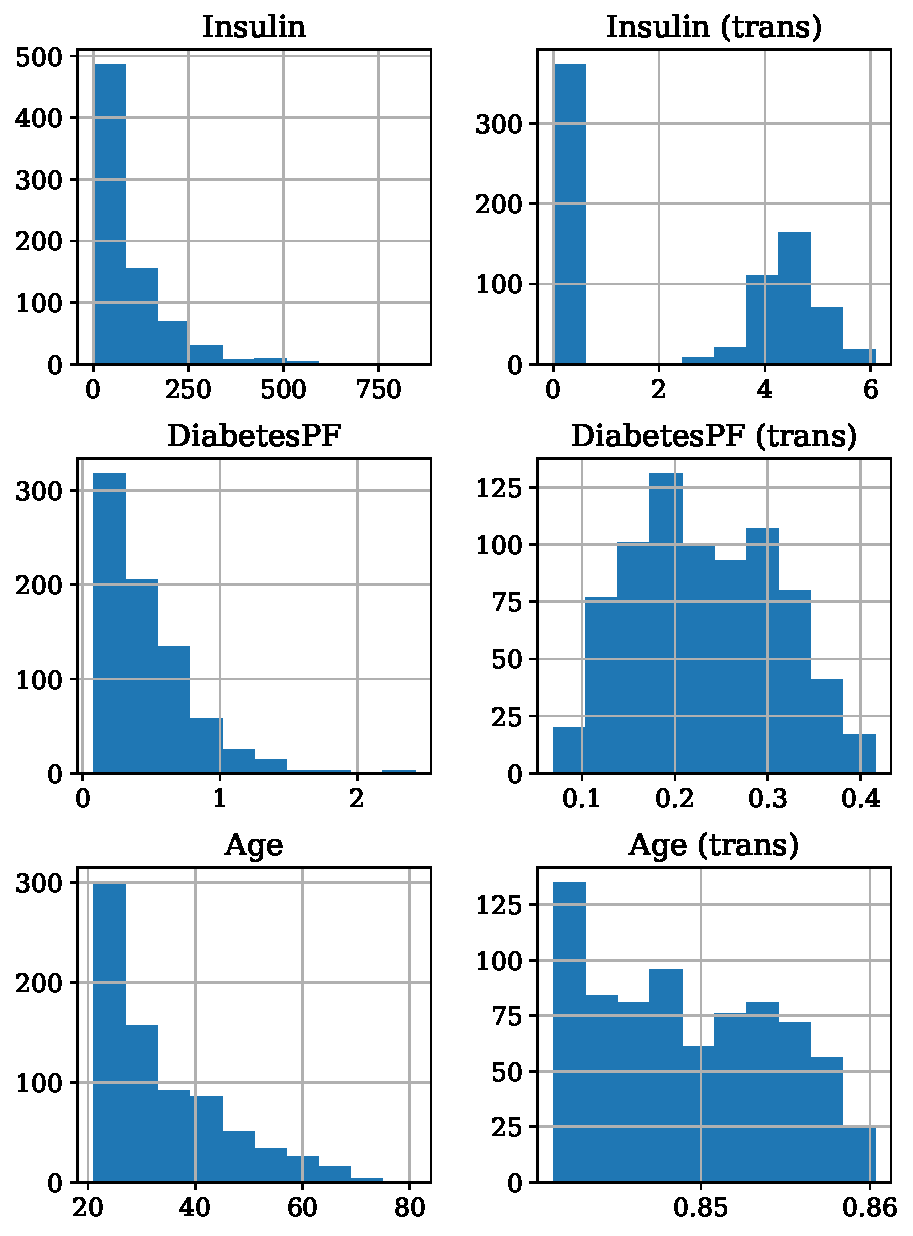
\includegraphics[width=0.4\textwidth]{figures/dist.pdf}
\vspace{-0.3cm}
\caption{The original and transformed distributions of the three most skewed features of the Pima Indians Diabetes Dataset}
\label{skew_dist}
\end{figure}
\begin{figure}[t]  % H
\centering
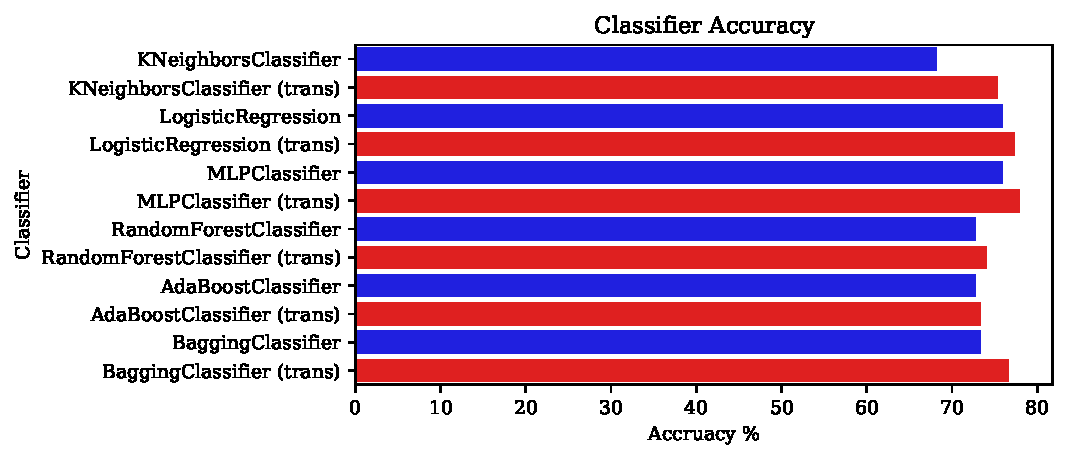
\includegraphics[width=0.5\textwidth]{figures/classifiers.pdf}
\vspace{-0.7cm}
\caption{The model accuracy of different classifiers based on the original (green bars) and transformed (red bars) distributions of the three most skewed features of the Pima Indians Diabetes Dataset}
\label{skew_acc}
\end{figure}

\begin{figure*}[!ht]  % H
	\centering % width=\textwidth
	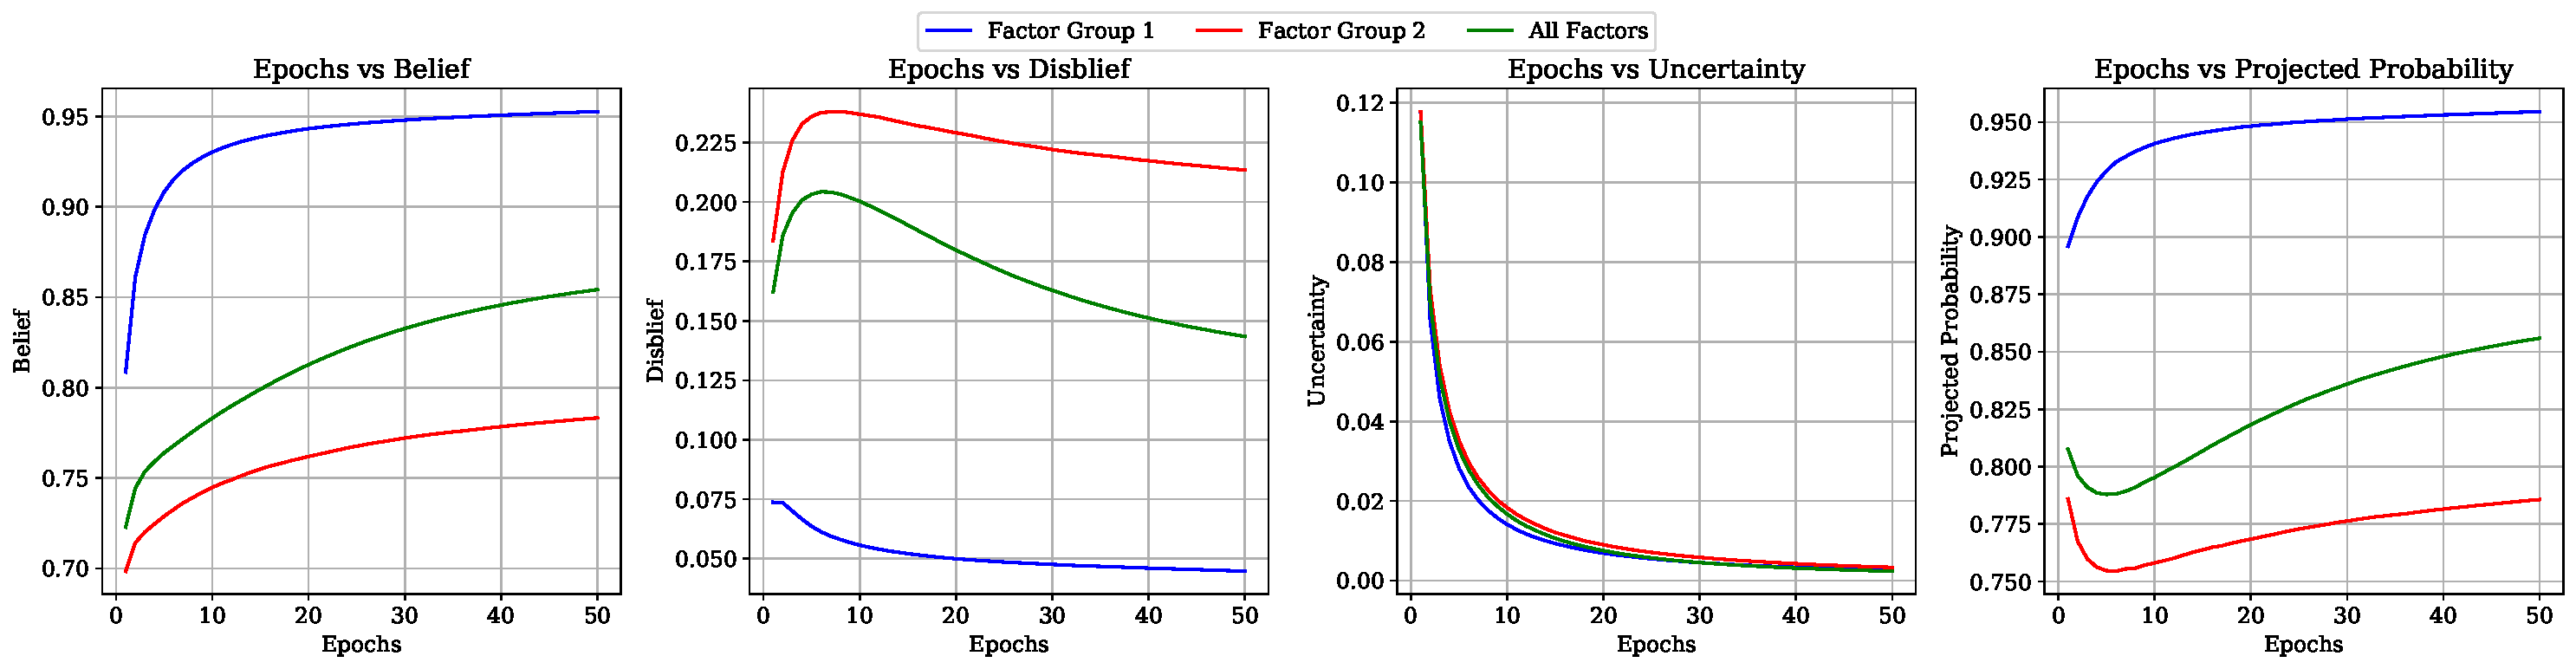
\includegraphics[width=0.8\textwidth]{figures/Results_Op_susy.pdf}
	\vspace{-0.3cm}
	\caption{The average improvement process of opinion determinants during 50 training epochs over 5 different runs based on different factors in numerical features for SUSY dataset}
\label{susy_op}
\end{figure*}
\begin{figure*}[!ht]
	\centering % width=\textwidth
	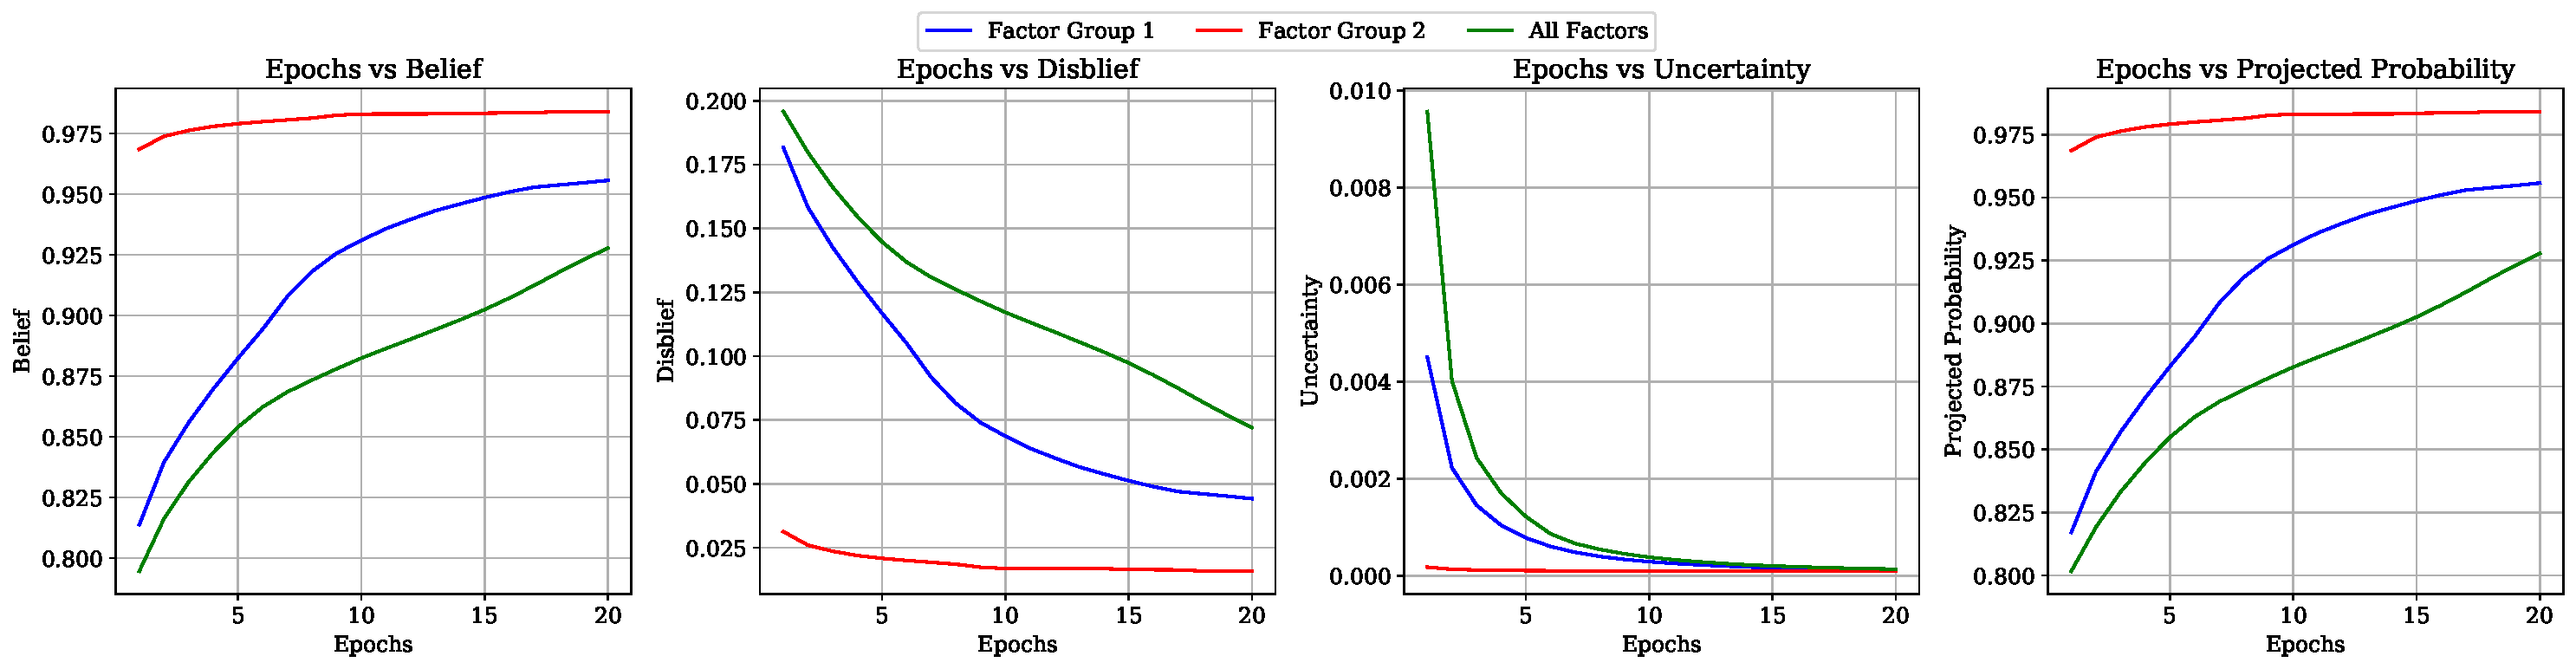
\includegraphics[width=0.8\textwidth]{figures/Results_Op_kdd.pdf}
	\vspace{-0.3cm}
	\caption{The average improvement process of opinion determinants during 20 training epochs over 5 different runs based on different factors in numerical features for KDD CUP 99 dataset}
\label{kdd_op}
\end{figure*}

The results show that the transformed feature distribution mitigates the skewness and kurtosis as two distributional properties of training data. We can see the accuracy improvement of all classifiers in the presence of transformed features. Therefore, the skewed training data features that also have higher kurtosis, can negatively impact the DNN performance. This result also indicates the necessity of considering statistical and distributional properties of input data in initializing data opinions before propagation through the DNN network.
}

\noindent \textbf{Main Experiments.} Since the datasets used to train DNN models can be considerably different in terms of their statistical properties, we used the equally-weighted average of two distinct groups of statistical factors for each data opinion determinant in each dataset. We run the experiment for two groups of statistical factors mentioned in Section~\ref{op_init_sec}. 
% Cronbach's Alpha, Data Quality Score (DQS), and Eigenvalue ratio (explained variance) as the first group and Skewness, Kurtosis, and the Distributional Variance as the second group. 
We first run the experiment for each group of factors separately and then together. In Figures~\ref{susy_op} and~\ref{kdd_op}, there are two lines, blue and red, indicating the change in model opinion determinants as well as the model projected probability considering the first and second group of data opinion initialization factors, respectively. The green line also indicates the change in model opinion determinants and its projected probability considering both sets of factors simultaneously, by the equally-weighted average. During training epochs, in Figures~\ref{susy_op} and~\ref{kdd_op}, we can see the increasing change in model belief as well as the decreasing change in model uncertainty for both datasets considering different factors separately and together.{\color{blue} Therefore, model belief and uncertainty are relatively improved during training epochs in a way that belief is increased while uncertainty is decreased. Finally, we can observe that during the training process, the model trustworthiness or projected probability is increased when there is no significant increasing change in disbelief. 

As the results show, arbitrary selection of statistical factors to initialize the input data opinions may impact the total model trustworthiness. Therefore, this approach is flexible enough in selecting different statistical factors based on the application, data type, research domain, and the objective of the classification task. However, using the weighted average of the most correlated factors in initializing each determinant of interpretable data opinions will lead to a more realistic view of the model trustworthiness because of considering more aspects of data distribution in a batch of training data. Note that as mentioned before, we use equally-weighted average of distinct factors in initialization process. Therefore, based on the application and task domain, different weights can be assigned to different factors for averaging to tune the importance and priority of some specific statistical factors.}

{\color{blue}
Furthermore, Figures~\ref{susy_loss} and~\ref{kdd_loss} illustrate that the training processes over both SUSY and KDD Cup 99 datasets are performed effectively as decreasing loss and increasing accuracy during the training process shown in these figures is a sign of a successful learning process.}
%(see Appendix~\ref{train_app})
A successful training process leads to an increase in model belief and projected probability as a measure of trustworthiness for both datasets while our model uncertainty is decreasing significantly. Thus, the projected probability is positively correlated with the model performance, and we can trust the DNN model much more than before after a successful training process. In comparison with the other trained models in the case of similar accuracy, we can decide to select the model with a higher projected probability at first, and in case of no significant discrepancy, the model with higher belief, lower disbelief, and lower uncertainty will be selected. In addition, we see insignificant change in the amount of disbelief (approximately less than 0.1) during training, which is convincing since our input data that fed to the DNN were of high quality without data type mismatch or any missing or misleading data records. 

{\color{blue} The low-quality input data may have missing and misleading data points or data type mismatch that give rise to input data with higher disbelief and lower trustworthiness. In Figures~\ref{susy_miss} and~\ref{kdd_miss}, we demonstrate the behavior of the proposed method in the presence of input data with lower quality. In this regard, we experiment the proposed method on both datasets with different ratios of missing/misleading data points. The results show that the lower quality input data with lower trustworthiness have higher model disbelief along with an increase in model disbelief during training rather than input data with higher quality. Therefore, we can observe that the more missing/misleading data ratios are in the datasets, the more model disbelief and the less model belief and trustworthiness (projected probability) we achieve during training epochs. We can also observe that low-quality data with lower trustworthiness may decrease the model belief and eventually, decrease the model trustworthiness during the training phase.         
}

We report the average performance results as well as initial and ultimate model opinions during five distinct runs for each dataset in Table~\ref{result}. In this table, the model opinion determinants for training and testing phases over each dataset are updated and improved based on the loss function and accuracy achieved during a total number of training epochs. Note that the total belief and projected probability or trustworthiness of the model have been increased compared to the first epoch of training while the uncertainty has been relatively decreased. This result confirms the impact of successful training and loss optimization on the quantification and propagation of the total opinion's determinants. 
% As the loss function is being minimized during training epochs, the accuracy of the entire network is increasing. Therefore, the model accuracy in training time is correlated to the belief and uncertainty of the model opinion. 
% Since the opinion determinants have an additivity requirement, change in one determinant coincides with changes in other determinants. 
% We can also see the improvement in the trustworthiness or projected probability of the model while training is performed. Note the difference between the projected probability in total opinion (after training) compared to the first epoch of training such that the total projected probability of the model has been increased compared to the starting point of training. Note that we could achieve better performance by hyperparameter tuning and/or increasing the number of training epochs. However, this improvement was irrelevant to the objectives of the experiment.  

\begin{table*}[!ht]
% \hskip -1.3cm
\centering
\caption{The average performance and opinion results for training and testing phases during 5 different runs over each dataset}
\vspace{-0.1cm}
\begin{tabular}{c c cccc cccc}
    \toprule
\multirow{2}{*}{\textbf{Dataset}} 
        & \multicolumn{1}{c}{\textbf{Performance}} & \multicolumn{4}{c}{\textbf{1st Training Epoch Opinion}} &
        \multicolumn{4}{c}{\textbf{Total Opinion}} \\
    \cmidrule(lr){2-2} \cmidrule(lr){3-6} \cmidrule(lr){7-10}
        & Total Accuracy & Belief & Disbelief & Uncertainty & Proj. Prob. & Belief  & Disbelief & Uncertainty & Proj. Prob. \\
    \midrule
SUSY: \textit{Training} 
        & 72.863\%  & 0.6420 & 0.0160 & 0.3420 & 0.8130 & 0.8470 & 0.0080 & 0.1440 & 0.9640      \\
    \addlinespace
SUSY: \textit{Testing}
        & 69.785\%   & - & - & - & - &  0.8495 & 0.0089 & 0.1417 & 0.9203        \\
    \addlinespace
KDDCup99: \textit{Training}
        & 99.065\%  & 0.9280 & 0.0050 & 0.0670 & 0.9610 & 0.9978 & 0.0002 & 0.0021 & 0.9981 \\
    \addlinespace
KDDCup99: \textit{Testing}
        & 97.846\%   &  -   &  -  &  -  & - &  0.9969 & 0.0002 & 0.0029 & 0.9970    \\
    % \addlinespace

% \multirow{4}{*}{KDD Cup 99}
%         & item 1    & item 2    & then 3    & item 4    & item 5    & item 6            \\
%         & item 1    & item 2    & then 3    & item 4    & item 5    & item 6            \\
%         & item 1    & item 2    & then 3    & item 4    & item 5    & item 6            \\
%         & item 1    & item 2    & then 3    & item 4    & item 5    & item 6            \\
    \bottomrule
\end{tabular}
%\vspace{-0.5cm}
\label{result}
\end{table*}

% In addition, any suitable value for each hyperparameter in our model like the number of required training epochs for convergence, the initial amount of learning rate, and the optimization approach can be leveraged to achieve the best possible accuracy.

In conclusion, our evaluation demonstrates that the opinion quantification process is adequately flexible when statistical properties of the input data are incorporated into the process. Note that the selection of these statistical factors can be different from one model to another based on the characteristics of the application domain. For example, in the medical domain, the reliability of input data could be a major factor in the opinion generation while in another domain, the skewness or kurtosis of data can have higher priority to be considered.

%Another advantage of incorporating statestical poroperties of input data in opinion propagation is its contribution to the interperqatbility and explainability of the  is the 


%charactristicsstatistical properties of the input dataset. These independent factors for data opinion initialization should be explainable and interpretable based on the nature of feature distributions, the task objective, and the application domain. We can also apply different weights for different factors in the proposed approach to tune the impact of each factor in initializing data opinion determinants. 

%the proposed data opinion propagation approach is adequately flexible for different DNN architectures.

%since based on the nature of input data and its features, any appropriate architecture of neural network can be utilized to train the model and achieve the best possible performance. 

%initialization approach for data feature opinions is constructed based on statistical properties of input data, also comprehensively flexible. Everyone can exploit and add more different and independent statistical factors, combined by weighted average, to initialize the data opinion determinants, even for the categorical features' opinions as well. 

\begin{figure}[ht]  % H
\centering
% \vspace{-10cm}
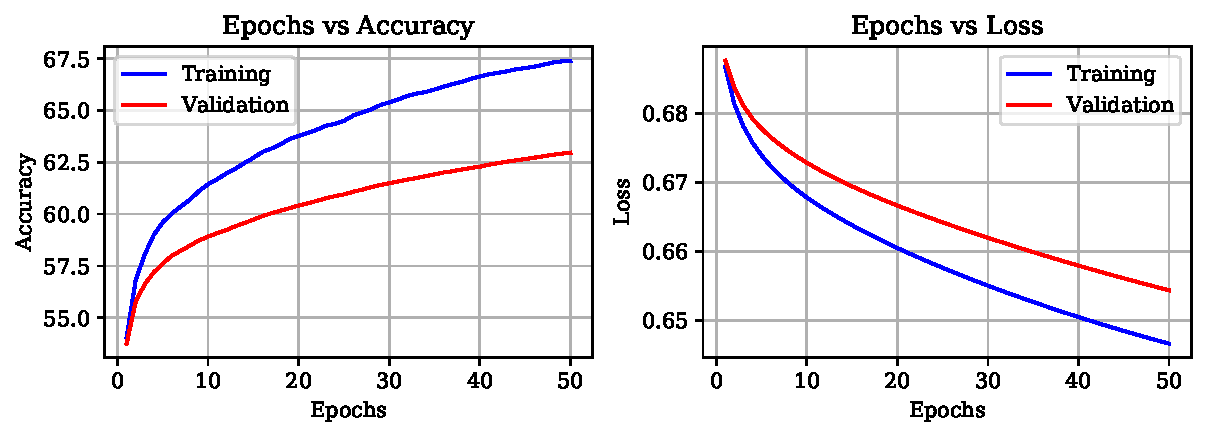
\includegraphics[width=0.5\textwidth]{figures/Results_susy.pdf}
%\vspace{-0.3cm}
\caption{The accuracy and loss values for training and validation phases during 50 training epochs over SUSY dataset}
\label{susy_loss}
\end{figure}

\begin{figure}[ht] % H
\centering
% \vspace{-22cm}
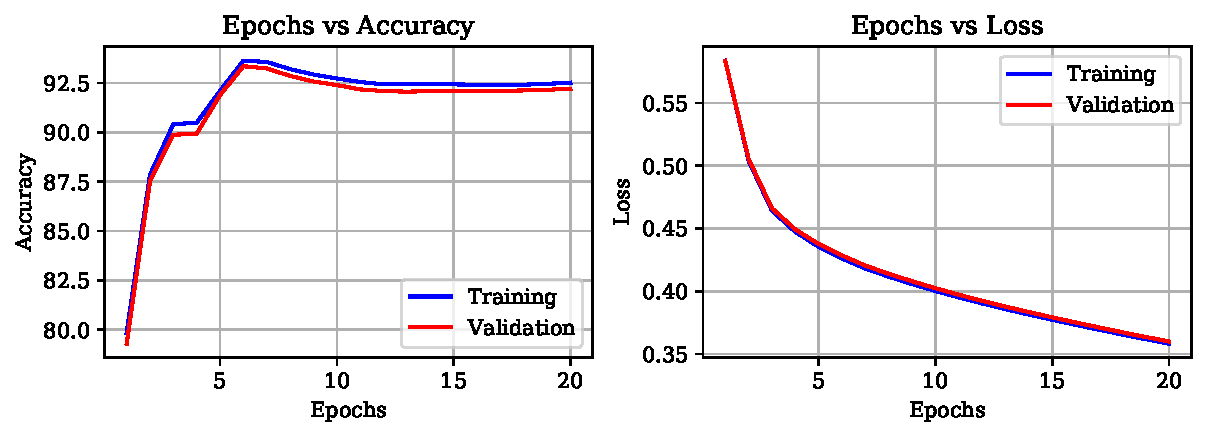
\includegraphics[width=0.5\textwidth]{figures/Results_kdd.pdf}
%\vspace{-0.3cm}
\caption{The accuracy and loss values for training and validation phases during 20 training epochs over KDD CUP 99 dataset}
\label{kdd_loss}
\end{figure}

\begin{figure*}[!ht]  % H
	\centering % width=\textwidth
	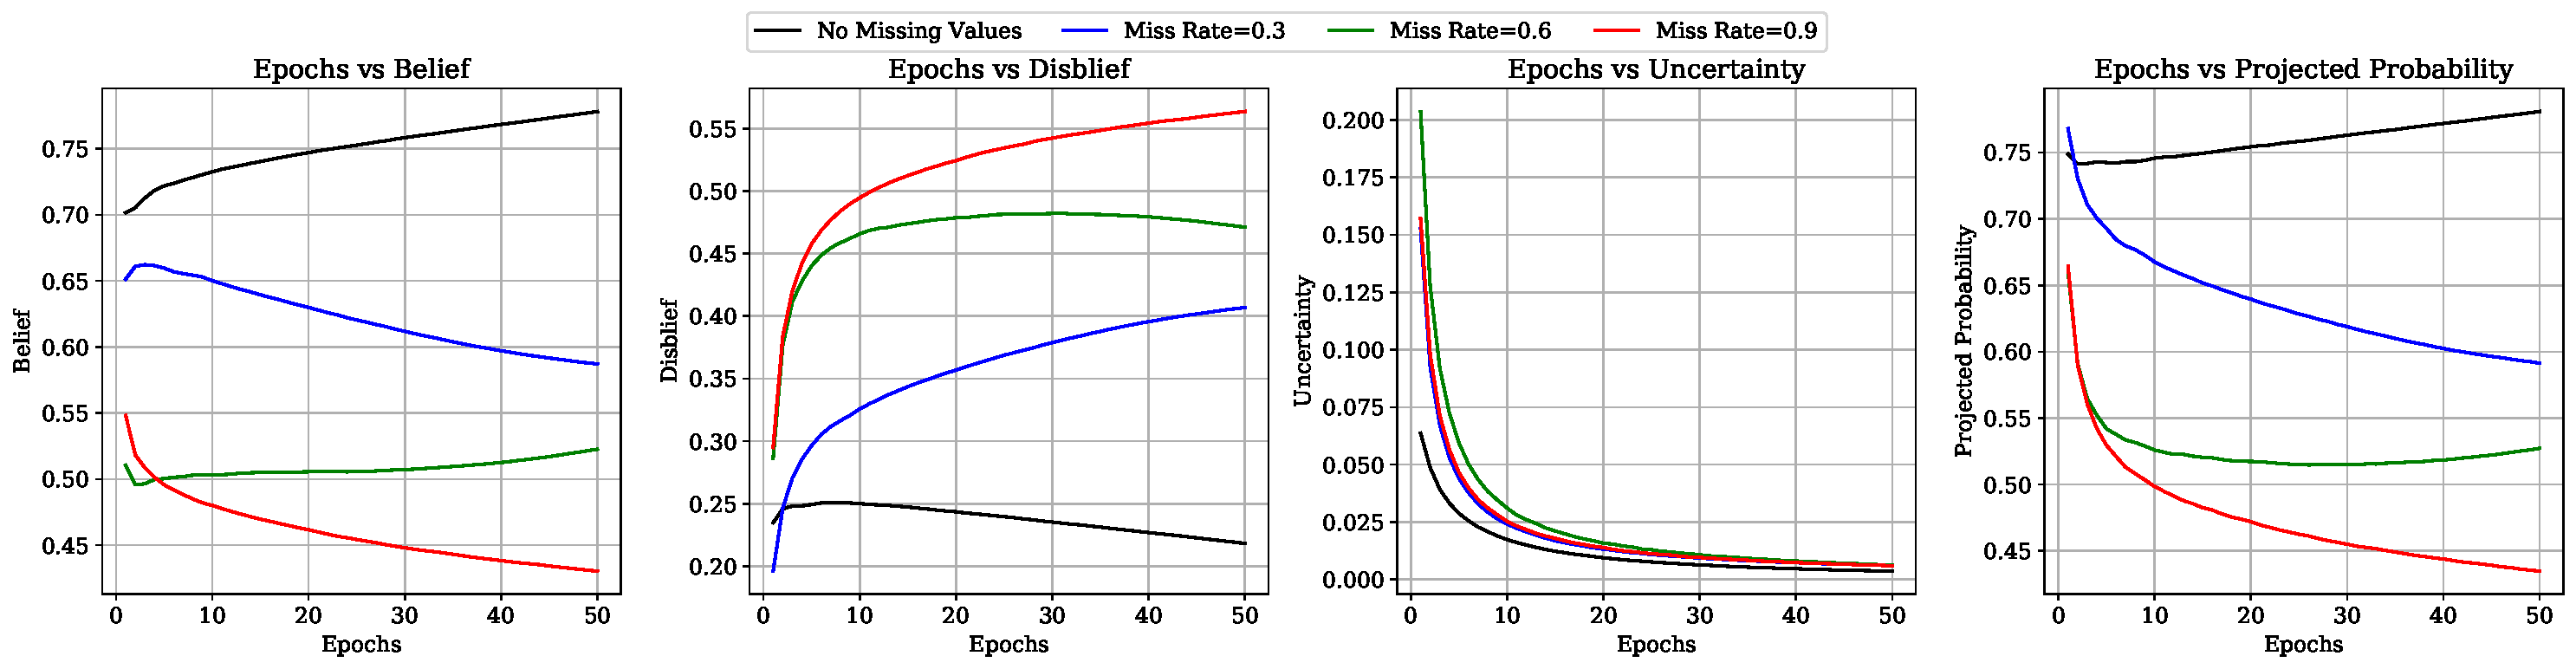
\includegraphics[width=0.8\textwidth]{figures/Results_susy_miss.pdf}
	\vspace{-0.3cm}
	\caption{The improvement process of opinion determinants during 50 training epochs over training data with different level of trustworthiness based on different miss rate for SUSY dataset}
\label{susy_miss}
\end{figure*}

\begin{figure*}[!ht]
	\centering % width=\textwidth
	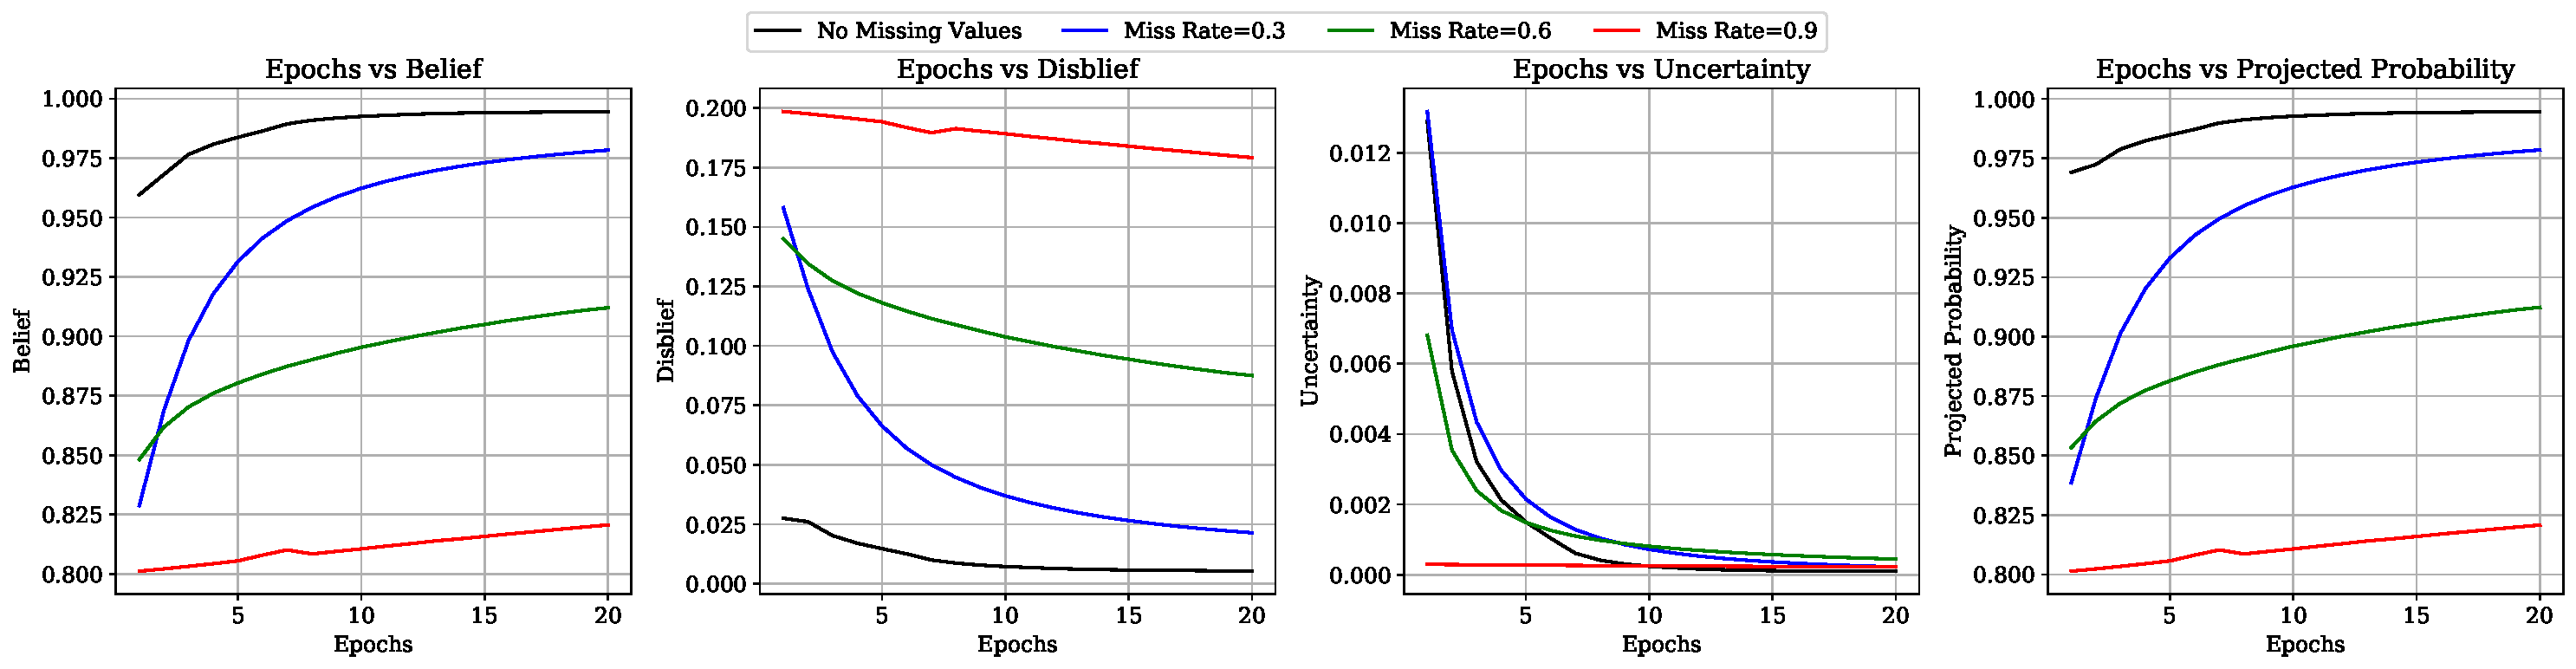
\includegraphics[width=0.8\textwidth]{figures/Results_kdd_miss.pdf}
	\vspace{-0.3cm}
	\caption{The improvement process of opinion determinants during 20 training epochs over training data with different level of trustworthiness based on different miss rate for KDD CUP 99 dataset}
\label{kdd_miss}
\end{figure*}









% Confusion matrices in the Figure~\ref{susy_cm} and~\ref{kdd_cm} demonstrate that the trained model could achieve good results and acceptable accuracy over unseen data (test data).

% \begin{figure}[H]
% 	\centering
% 	\includegraphics[scale=0.5]{figures/susy_cm.PNG}
% 	\caption{A Confusion matrix for testing over SUSY dataset}
% 	\label{susy_cm}
% \end{figure}
% \begin{figure}[H]
% 	\centering
% 	\includegraphics[scale=0.5]{figures/kdd_cm.PNG}
% 	\caption{A Confusion matrix for testing over KDD Cup 99 dataset}
% 	\label{kdd_cm}
% \end{figure}


%%%%%%%%%%%%%%%%%%%%%%%%%%%%%%%%%%%%%%%%%%%%%%%%%%%%%%%%%%%%%%%

% \usepackage{booktabs, multirow}


% \begin{table}
% \centering
% \begin{tabular}{c ccc ccc}
%     \toprule
% \multirow{2}{*}{two rows} 
%         & \multicolumn{3}{c}{3-columns cell} & \multicolumn{3}{c}{3-columns cell}   \\
%     \cmidrule(lr){2-4} \cmidrule(lr){5-7}
%         & column 1  & column 2  & column 3  & column 4  & column 5  & column 6          \\
%     \midrule
% \multirow{4}{*}{Social Network}  
%         & item 1    & item 2    & then 3    & item 4    & item 5    & item 6            \\
%         & item 1    & item 2    & then 3    & item 4    & item 5    & item 6            \\
%         & item 1    & item 2    & then 3    & item 4    & item 5    & item 6            \\
%         & item 1    & item 2    & then 3    & item 4    & item 5    & item 6            \\
%     \addlinespace
% \multirow{4}{*}{Citation Dataset}
%         & item 1    & item 2    & then 3    & item 4    & item 5    & item 6            \\
%         & item 1    & item 2    & then 3    & item 4    & item 5    & item 6            \\
%         & item 1    & item 2    & then 3    & item 4    & item 5    & item 6            \\
%         & item 1    & item 2    & then 3    & item 4    & item 5    & item 6            \\
% \bottomrule
% \end{tabular}
% \caption{Example of professional table design}
%     \end{table}


% \begin{table}[t]
% \begin{tabular*}{\columnwidth}{@{\extracolsep{\fill}}%
%     l T{4}T{2}T{2}T{4}}
% \toprule
% Year & {Nones}& {Option 1} & {Option 2} & {Total} \\
% \midrule
%   2001& 126   & 16    & 2     & 144 \\
%   2002& 114   & 9     & 4     & 127 \\
%   2003& 115   & 7     & 1     & 123 \\
%   2004& 114   & 6     & 4     & 124 \\
%   2005& 104   & 5     & 8     & 117 \\
%   2006& 96    & 3     & 6     & 105 \\
%   2007& 93    & 2     & 4     & 99 \\
%   2008& 93    & 2     & 2     & 97 \\
%   2009& 85    & 2     & 11    & 98 \\
%   2010& 83    & 0     & 7     & 90 \\
%   2011& 74    & 0     & 12    & 86 \\
%   \midrule
%   Total & 1097 & 52   & 61    & 1210 \\
% \bottomrule
% \end{tabular*}
% \end{table}



% \begin{table*}
% %
% \tablestyle[sansbold]
% %
% \begin{tabular}{*{2}{p{0.45\textwidth}}}
% \theadstart
%     \thead header &
%     \thead header \\
% \tbody
%  %
%  content  & content \\
%  content  & content \\
%  content  & content \\
%  %
%  \tsubheadstart
%  \tsubhead subhead &
%  \tsubhead subhead \\
%  %
%  content  & content \\
%  content  & content \\
%  \tend
% \end{tabular}
% \vspace{2mm}
% \caption{sansbold style}
% \label{tab:style:sansbold}
% \end{table*} 
\section{Related Work}
\label{relw}
There are several uncertainty quantification approaches in deep learning that intend to quantify the concept of trust or uncertainty in neural networks. Bayesian DNNs that learn weights' distribution, are the state-of-the-art techniques for predictive uncertainty estimation~\cite{uncer1,dropout,ensemble,uncer_baseline,clara}. The Bayesian DNNs are computationally expensive compared to non-Bayesian (standard) DNNs. 
% CLARA is a framework developed by Facebook using Bayesian probabilistic model to aggregate reviewer decisions and predicted labels to measure uncertainty~\cite{clara}. 
In addition, there is no method proposed in these studies to measure the trustworthiness of parties which is vital in consensus tasks. In regular DNNs, there are some methods for quantifying trust in the learning models. For instance, in~\cite{break}, the authors introduce a new trust quantification approach based on a descriptive matrix called Trust Matrix as a complement to their previous work~\cite{wong1} and~\cite{wong2}. However, in case of low confidence and incorrect prediction, a substantial trust value can be seen which is not convincing, and the remedy suggested for this issue can cause more cost and complexity for the whole system. Subjective logic is also another approach used by~\cite{reput_uncer,uncer2,uncer3} to consider second-order uncertainty and trustworthiness in their learning systems. A closely related work is a proposal by Cheng et al.~\cite{hope} that exploits Subjective Logic~\cite{sl} to produce subjective opinions of a DNN to quantify trust in multi-layer neural networks. They introduce a quantification method named DeepTrust, as a framework based on Subjective Logic in which the model opinion and trustworthiness are quantified. Our proposal can be considered as an extension of the work of~\cite{hope} where we studied the limitations of the current method (see Section~\ref{limit}) and extended the method to incorporate interpretable input data opinions.  
%to be propagated in a DNN model to quantify model trustworthiness. 


% They showed that the consensus achieved by CLARA, is better than using majority voting approach; however, there is no method to measure trustworthiness of parties which is so important in consensus tasks.


% By answering a set of predefined questions (input data), Wong et al. provided and introduced some metrics to evaluate the overall amount of trust in DNNs~\cite{wong1}. These questions and answers so as to quantify trustworthiness are based on the behaviors of actors and their amount of confidence when they provide their responses due to being overconfident or conservative since due to related psychological history, the trust is partially associated with the amount of confidence. 

% The default state that they consider for their data is balanced, however, we do not know whether data being balanced or imbalanced has impact on the amount of trust or not which it probably does not have any impact on it. Furthermore, the work in the result section suffers from lack of comparison with any other DNNs or models, and just a row of result information is provided. Moreover, there is a discussion on unfairness between some demographic groups but just based on the their provided diagrams; however, it needs more justification or at least more information about data for their unfairness to be implicated like the scenario in which maybe the number of members in each demographic group vary and are unbalanced relative to each other to give rise to this unfairness.

% There are several research on using decentralized FL to create improved private framework for communicating among clients and models to obtain a general optimized model with respect to an acceptable performance.
% Recently,~\cite{bellet},~\cite{koloskova}, and~\cite{vanha} are three instances of the most important research work on peer-to-peer FL which they have utilized a fully decentralized SGD framework based on learning personalized models collaboratively with asynchronous clients’ activity. In~\cite{bellet} and~\cite{cyffer}, the goal is to achieve better trade-offs between performance and privacy in decentralized FL by improving scalability across clients or amplifying differential privacy guarantees based on appropriate relaxations of local differential privacy. However, these studies do not propose any trust quantification to measure trustworthiness or any determinants of trust in their networks in neither clients’ view nor communications’ view. Also, they suffer from network constraints and peer-to-peer costly communication limitations which this specific problem is addressed and relatively mitigated in~\cite{leasgd}.

% In~\cite{shrid}, Shridhar et al. tried to estimate uncertainty in form of probability distribution using Bayesian neural network as well as being more robust to overfitting. Nevertheless, regarding probabilistic reasoning, there is a need on how the uncertainty can be decreased to allow the decisions made by the network to be more confident and deterministic by growing in data size~\cite{mcadv}. In addition, in~\cite{zante}, the authors learn the similarity graph by connected components over clients as well as personalized model using sparse updates communications. However, robustness to malicious clients or the presence of unreliable data or labels are considered as an important gap. Thus, using some mechanisms incorporating decentralized FL will be a rising prominent goal which is hard to gain without a central trusted server~\cite{mcadv}. In this regard, the questions will be what kind of trusted central authority is required to setup the task in decentralized FL, and how we can determine it.

% Although using Secure Multi-party Communication as well as some state-of-the-art approaches such as secure aggregation and shuffling can be very beneficial to obtain better privacy level and performance trade-off, it is computationally expensive and also, we still need an approach to quantify trust or its determinants in decentralized FL setup to be vigorous enough in detecting or identifying malicious and unreliable clients or in case of any potential collusion~\cite{mcadv}.


%'a probabilistic logic description of a DNN by considering trust in both sides of the system, input dataset and inner functional operations. This approach is almost fully dependent on background knowledge of the input dataset like given opinions, trust information, and quality of initial data and labels.
%%% Our Contribution
% Therefore, according to the aforementioned gaps, the first part of our contribution is to devise an approach to initialize the input data opinions based on statistical and interpretable properties of training data. This quantification can provide a base infrastructure to quantify generalized trust measurement in decentralized FL based on different human norms of trust.
%%% Future Contributions %%%
% Minimizing uncertainty in each training round to reach an acceptable convergence in a decentralized FL system.
% Further Description: 
% Maximizing confidence and projected probability (which is a partial representation of trust based on a specific parameter). 
% Defining and devising a loss function. (bi-level optimization) (refer to non-linear programming: MIT press)
% This can be just one of the goals which will be the focus of this research and the rest will be considered as future work.

% Quantifying overall trustworthiness (according to its formal definition) in the form of a comprehensive subjective opinion (representation) based on various dependent determinants and human norms like performance, privacy, security, fairness, etc. in a decentralized FL system with respect to the amount of uncertainty.
% Just a quick mentioning: Using Dirichlet PDF and Multinomial Subjective Logic and investigating the possibility for any potential collusion.

% Detect and identify malicious or unreliable clients in decentralized federated settings based on different human norms. (application)
% Just a quick mentioning: Using quantified overall trust from previous step.




\section{Conclusion}
\label{conc}
% In this paper, we investigated the distributional changes in input data features can impact the model performance. we initialized the training data opinions to be propagated through the DNN using statistical and distributional properties of input data. Moreover, we improved the opinion optimization process by considering positive and negative evidence as well as uncertain evidence in model predictive outputs. We evaluated our proposed method using two real-world datasets, SUSY and KDD CUP 99, containing numerical and categorical features which are considerably different in terms of many statistical, natural, and domain aspects. Therefore, we observed that by decreasing loss and increasing accuracy during our training epochs, the amount of belief and trustworthiness (projected probability) are increasing while our model uncertainty is decreasing significantly. We also demonstrate the impact of different statistical or conceptual factors of data opinion initialization over total model opinion’s determinants. As a future work, we are currently working on propagating data and model opinions through a decentralized federated settings in which different client models are trained by their local data to achieve an improved global model. 
% We intend to quantify the total uncertainty of a federated network based on propagated clients’ opinions over a specific amount of training rounds. Therefore, we utilize our approach in each communication, aggregation, and propagation activities in federated learning without a significant computational cost.
In this paper, we investigated the limitations of the state-of-the-art opinion propagation method to quantify model trustworthiness. We proposed a new approach to initialize input data opinions by interpretable statistical metrics based on intrinsic properties of training data. To initialize the numerical, categorical, and target features, we selected distinct statistical properties originated in input data feature distributions. We also improved the opinion optimization process by considering uncertain evidence in forming the error opinion. Finally, we demonstrated the impact of input data distribution on the model performance and evaluated our proposed data opinion propagation method over two real-world datasets. Our experimental results confirmed that the model trustworthiness and performance are correlated such that the model belief and uncertainty are improved during the training process with respect to different data opinion initialization.   















% In this research, we utilized SL to propagate and measure the uncertainty in a decentralized federated learning system. This method is adequately flexible in different DNN architectures since it acts as an add-on in a ML system by being applied along with the training process in each DNN, therefore, it has no significant additional computational burden. It is also compatible with the state-of-the-art methods of communication amongst different DNNs.

% In this research, We leverage Subjective Logic as a tool and inject it to deep neural networks in order to propagate and measure the uncertainty in a single DNN, with an aim of propagating and quantifying total uncertainty in a decentralized federated learning system. Furthermore, using subjective logic in our proposed approach is fully beneficial and adequately flexible in different DNN architectures since it can act as an add-on in a ML system by being applied along with the training process in each DNN, therefore, it has no significant additional computational burden. It is also compatible with the state-of-the-art methods of communication amongst different DNNs. The objective of our research is to develop a novel method for propagating uncertainty associated with training dataset as subjective opinions through a DNN model leading to the total model opinion containing total model uncertainty. Thus, we exploit some statistical and conceptual method to quantify and initialize data uncertainty and opinions to be propagated based on the nature of input data features. During training process, the model updates its parameters' opinions and outputs its total opinion. Each feature or label opinion individually participates in training process. Therefore, for opinion propagation through a network, the opinions of data features and labels are separately initialized. 
% We evaluate our proposed method using two real-world datasets, SUSY and KDD CUP 99, containing numerical and categorical features which are considerably different in terms of many statistical, natural, inferential, and domain aspects. Based on our evaluation, we expect a DNN model with higher accuracy indicates lower uncertainty. Therefore, we observe that by decreasing loss and increasing accuracy during our training epochs which is the sign of successful learning, the amount of belief is increasing while our model uncertainty is decreasing significantly. We show that the belief and uncertainty will be improved in a DNN model based on its loss function optimization during training process. Moreover, we indicate the impact of successful training and loss optimization on the total opinion and its determinants in the learning model. We also demonstrate the impact of different statistical or conceptual factors of data opinion initialization over total model opinion’s determinants like belief and uncertainty in a way that each opinion determinant is relatively improved during training epochs. As a future work, we are currently working on propagating data and model opinions through a decentralized federated settings in which we can train different client models over their private data without sharing confidential data information to achieve an improved global model. We intend to quantify the total uncertainty of a federated network based on propagated clients’ opinions over a specific amount of training rounds. Therefore, we utilize our approach in each communication, aggregation, and propagation activities in federated learning without a significant computational cost.




% \input{sections/}
% \input{sections/}
% \input{test}

%\section*{Acknowledgment}


% References
\bibliography{references}
\bibliographystyle{IEEEtran}    % \bibliographystyle{alpha}


% NOTE: necessary when ptmx or no mathfont class option is given
% \providecommand{\upGamma}{\Gamma}
% \providecommand{\uppi}{\pi}
\appendices
% \begin{appendices}
\section{Single Deep Neural Network}
\label{dnn_app}
A Deep Neural Network (DNN) is a computational network that can be considered as a function $\mathcal{M}_\Theta:~\mathcal{D} \rightarrow \hat{Y}$ in which $\mathcal{D}$ is a set of input data fed into the network, $\Theta$ is a set of network parameters (weights and biases), and $\hat{Y}$ is the output set of the approximated values $\hat{y} \in \hat{Y}$. Moreover, the DNN model $\mathcal{M}_{\Theta}$ aims to be trained based on its input data (a finite set of training data) denoted by $\mathcal{D}$, according to the function~$\mathcal{Q}:~\mathcal{D}~\rightarrow~Y$ such that, 
\[
\mathcal{Q} = \{\ (d_{i},y_{i})\ |\ i \in \mathbb{N}^{[1,m]}\ \}\ ,
\]
where $i$ is a data point with $d_{i}$ and $y_{i}$ representing features and target labels, respectively and $m$ is the number of participating data points (data samples) in the training dataset.

In the DNN model $\mathcal{M}_{\Theta}$, we intend to optimize a loss function in the form of $\mathcal{L}(\mathcal{D},\Theta;Y)$. This optimization is performed by minimizing the average of each data sample $i$'s loss value with respect to the parameter set of $\Theta$ defined as, 
\begin{equation}
\min_{\Theta}\ \mathcal{L}(\mathcal{D},\Theta;Y) = \frac{1}{m}\ \sum_{i=1}^{m} loss(d_{i},\Theta;y_{i})\ ,
\label{loss}
\end{equation}
where $loss(d_{i},\Theta;y_{i})$ is the loss function of the single data sample $i$ in the training dataset.

\section{Opinion Determinants in Subjective Logic}
\label{sl_app}
\vspace{.2cm}
\noindent\textbf{Definition 1 (Belief and Disbelief Masses).} The belief $b$ and disbelief $d$ are the amount of being in support of and against the truth of a particular subjective variable in a DNN provided by a DNN component, respectively~\cite{sl}. % $\hfill \blacksquare$

\vspace{.2cm}
\noindent\textbf{Definition 2 (Uncertainty Mass).} The uncertainty $u$ is the amount of not being confident (certain) or not having sharp idea regarding the truth of a subjective variable provided by a DNN component. The uncertainty is caused by vacuity of evidence in a DNN model. Thus, the fewer observations (data samples) may give rise to more uncertainty~\cite{sl}.% $\hfill \blacksquare$

\vspace{.2cm}
\noindent\textbf{Definition 3 (Base Rate Mass).} The base rate $a$ is the prior probability for a subjective variable that can be interpreted as a kind of bias term which provided by a DNN component. The base rate can help us take the bias measure into account~\cite{sl}. % $\hfill \blacksquare$

{\color{red} \section{Parameter Opinion Initialization}
\label{parint_app}
We initialize the model parameters opinions according to the lack (vacuity) of observations by Uncertainty Maximization~\cite{sl} on randomly generated opinions from uniform distribution $\mathcal{U}(0,1)$ with respect to the opinion additivity requirement~\ref{additivity}. In Uncertainty Maximization, an opinion for the parameter $\theta$ should have at least one belief mass of zero, i.e. $b_{\theta} = 0$ and the uncertainty is calculated as,
\begin{equation}
    u_{\theta} = \min(1,\frac{PP_{\theta}}{a_{\theta}})\ ,
\end{equation}
where $PP_{\theta}$ and $a_{\theta}$ is the projected probability and the base rate of the parameter $\theta$'s opinion, respectively.}

{\color{red}
\section{Parameters Opinion Update}
\label{opt_app}
To optimize the total opinion of our model (minimizing the uncertainty while maximizing the belief), we need to update the parameters' opinions based on the error value $|y-\hat{y}|$ that the model is achieving during training. Thus, we exploit back propagation approach for the parameters' opinion updates while we are updating the actual parameters in mini-batch gradient descent to minimize the loss function. Based on what we perform in back propagation process to update the parameters in each layer, we initialize the opinions of parameters' change, $O_{\Delta w}$ and $O_{\Delta b}$, backward from the last layer towards the first layer using error opinion set $O_{\delta}$ and its pairwise multiplication with predicted opinion set $O_{\hat{y}}$ in the previous layer. For instance, in layer $i$,
\begin{equation}
    O_{\Delta b}^i = O_{\delta} \qquad \textnormal{and} \qquad O_{\Delta w}^i = O_{\delta} \otimes O_{\hat{y}}^{i-1}\ .
\end{equation}

Finally, in each layer $i$ with the neuron set $layer_i$, we update the error opinion set $O_{\delta}$ by assigning a set consists of multi-source average fusion on the pairwise multiplication of the previous $O_{\delta}$ and the weight opinion set $O_{w}^i$ as follows:
\begin{equation}
    O_{\delta} = \{ \bigoplus_{layer_i}(O_{\delta}\ \otimes\ O_{w}^i)\ \}\ .
\end{equation}

Then, we update the opinion of each parameter $\theta$ denoted by $O_{\theta}$, by taking cumulative fusion on its previous opinion and its change opinion denoted by $O_{\Delta \theta}$, as follows:
\begin{equation}
    O_{\theta} = O_{\theta}\ \widehat{\oplus}\ O_{\Delta \theta}\ .
\end{equation}
}

{\color{red}
\section{Impact of Data Distribution on Model Performance}
\label{impact_app}
The objective of this preliminary experiment is to demonstrate how the distributional properties in input data can impact the model performance. We used Pima Indians Diabetes Dataset\footnote{\url{https://www.kaggle.com/datasets/uciml/pima-indians-diabetes-database}} originally from the National Institute of Diabetes and Digestive and Kidney Diseases. 

We apply classification task using different traditional classifiers like K-nearest, Logistic Regression, Random Forest, AdaBoost, and a DNN classifier (\emph{MLPClassifier} with three layers optimized by Adam and with initial learning rate of 0.01) on both original distributions (e.g. skewed) and transformed distributions (e.g., no longer skewed). 
%K-nearest, Logistic Regression, Random Forest, AdaBoost, and Bagging classifiers on the original and transformed data features. 
%For the DNN classifier, we used \emph{MLPClassifier} as a three-layer neural network model optimized by Adam and initial learning rate of 0.01. 
As shown in Figure~\ref{skew_dist}, the distribution of the three most skewed features of the dataset named \emph{Insulin}, \emph{DiabetesPedigreeFunction}, and \emph{Age} as well as the transformed features are shown. Therefore, in Figure~\ref{skew_acc}, we can see the accuracy of different classifiers including the DNN model over the original and transformed distributions of the most skewed features that hold the highest skewness and kurtosis in this dataset.
\begin{figure}[!ht]  % H
	\centering
	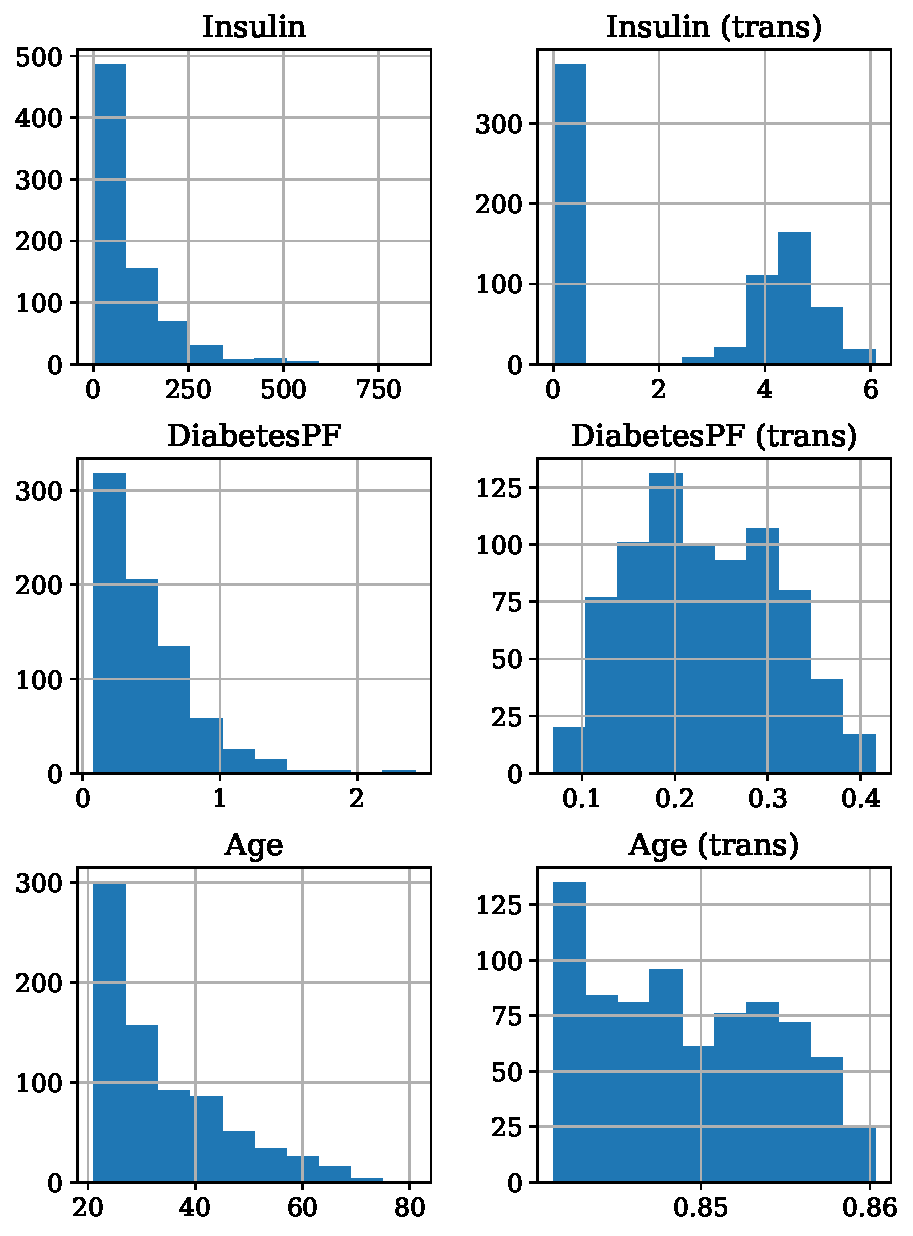
\includegraphics[width=0.4\textwidth]{figures/dist.pdf}
	\vspace{-0.3cm}
	\caption{The original and transformed distributions of the three most skewed features of the Pima Indians Diabetes Dataset}
%	\label{skew_dist}
\end{figure}
\begin{figure}[!ht]  % H
	\centering
	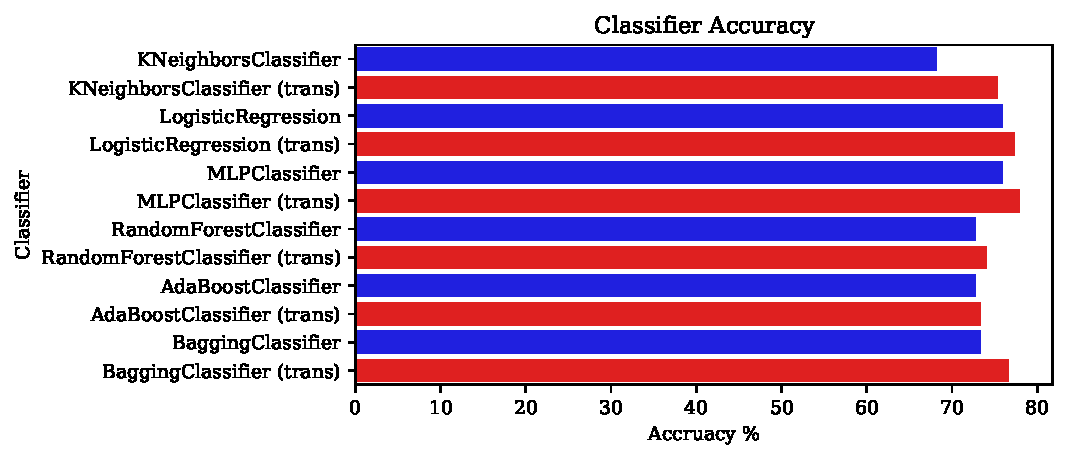
\includegraphics[width=0.5\textwidth]{figures/classifiers.pdf}
	\vspace{-0.7cm}
	\caption{The model accuracy of different classifiers based on the original (green bars) and transformed (red bars) distributions of the three most skewed features of the Pima Indians Diabetes Dataset}
%	\label{skew_acc}
\end{figure}
The results show that the transformed feature distribution mitigates the skewness and kurtosis as two distributional properties of training data. We can see the accuracy improvement of all classifiers in the presence of transformed features. Therefore, the skewed training data features, that have higher kurtosis as well, can negatively impact the DNN performance. This result also indicates the necessity of considering statistical and distributional properties of input data in initializing data opinions before propagation through the DNN network. 
}

{\color{red}
\section{Model Training}
\label{train_app}
Figures~\ref{susy_loss} and~\ref{kdd_loss} illustrate that the training process over both SUSY and KDD Cup 99 datasets has been performed effectively for both datasets as decreasing loss and increasing accuracy during the training process shown in these figures is a sign of a successful learning process. 
\begin{figure}[ht]  % H
	\centering
% 	\vspace{-10cm}
	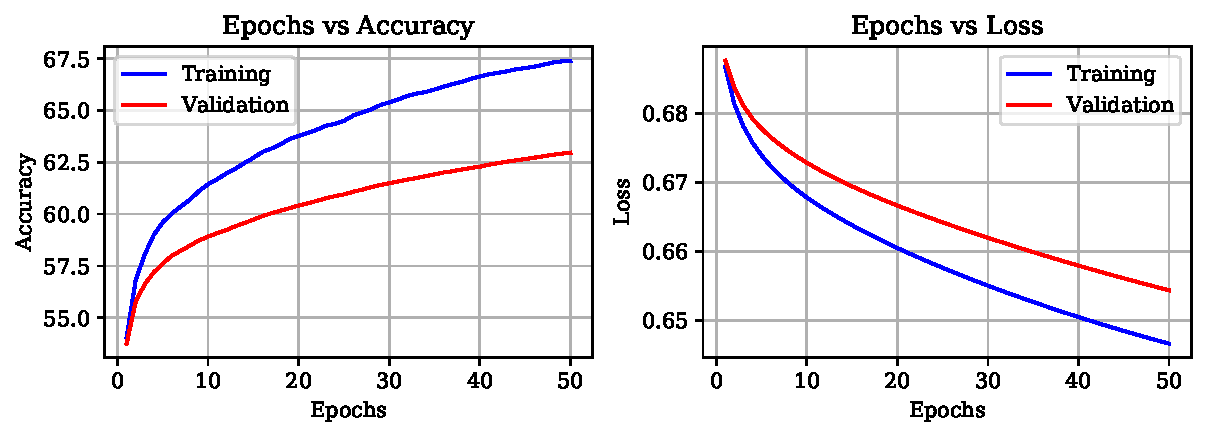
\includegraphics[width=0.5\textwidth]{figures/Results_susy.pdf}
	\vspace{-0.3cm}
	\caption{The accuracy and loss values during 45 training epochs over SUSY dataset}
%	\label{susy_loss}
\end{figure}
\begin{figure}[ht] % H
\centering
% \vspace{-22cm}
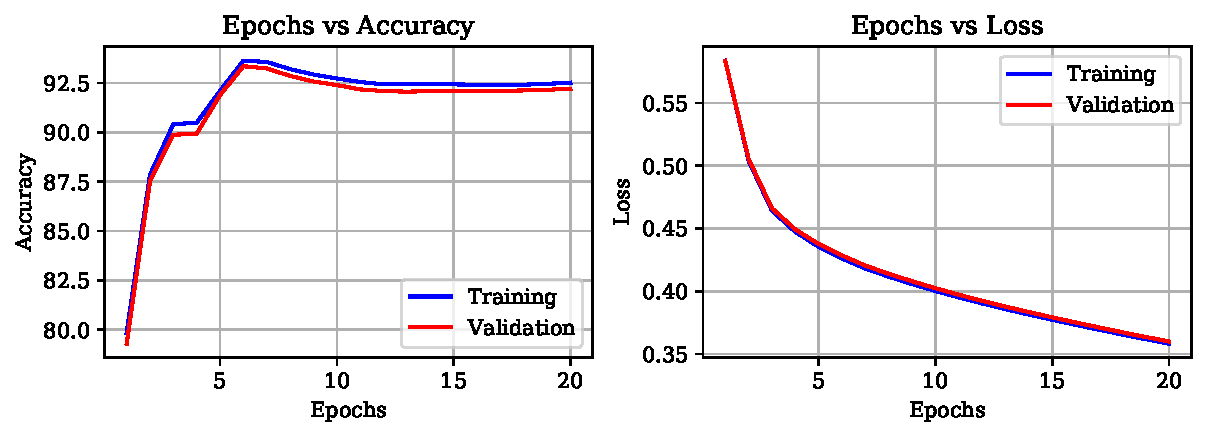
\includegraphics[width=0.5\textwidth]{figures/Results_kdd.pdf}
\vspace{-0.3cm}
\caption{The accuracy and loss values during 20 training epochs over KDD Cup 99 dataset}
%\label{kdd_loss}
\end{figure}
}

\section{Investigation on Optimal Thresholds in Opinion Optimization}
\label{thr_app}

{\color{blue} According to Equation~\ref{makeop}, in the opinion optimization process, we use two different thresholds $\phi_1$ and $\phi_2$ to determine the error opinion $O_\delta^l$ for each target label $l$. Thus, we need to find the optimal values for selecting the thresholds. In this regard, we applied the proposed method using Susy dataset on different selections of the thresholds with respect to their requirements mentioned in Section~\ref{op_opt}. Figure~\ref{susy_thr} shows the model opinion results during training using different selections of the two thresholds. We can observe that when $\phi_1=0.4$ and $\phi_2=0.7$ (the purple line), we see the higher amount of model belief and trustworthiness along with lower amount of disbelief rather than other choices of thresholds.
}
\begin{figure*}[t]  % H
	\centering % width=\textwidth
	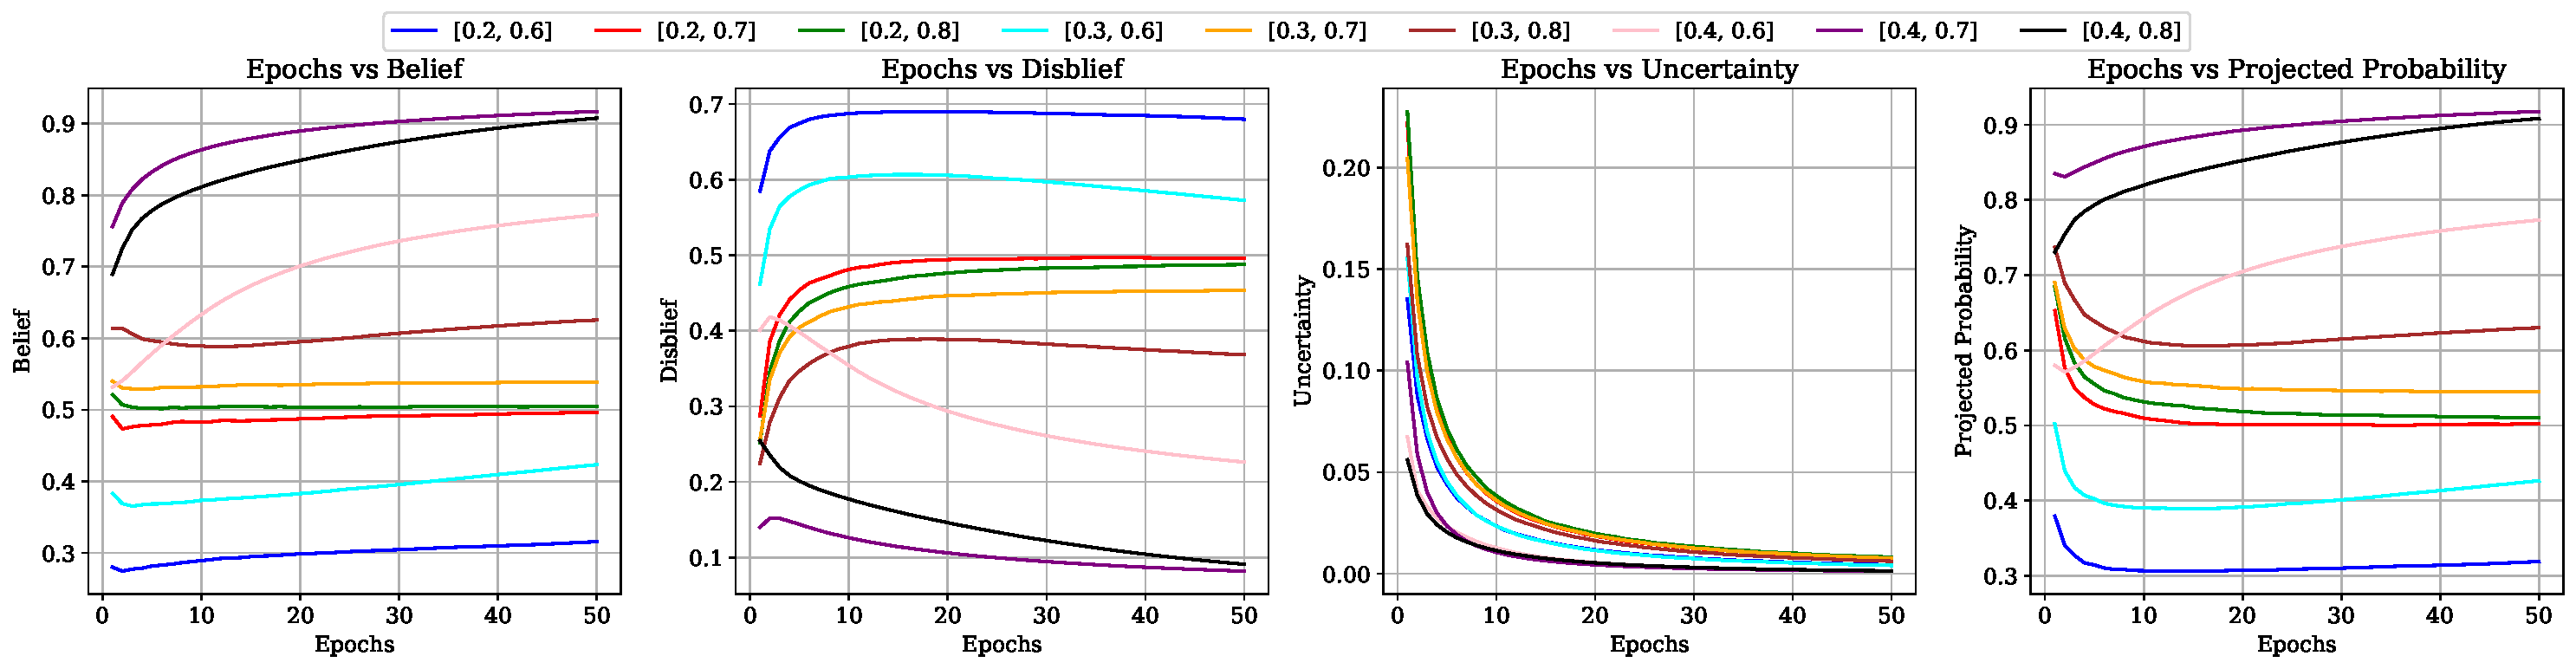
\includegraphics[width=0.8\textwidth]{figures/Results_susy_thr.pdf}
	\vspace{-0.3cm}
	\caption{The behavior of each determinant of total model opinion with respect to different selections of opinion optimization thresholds $\phi_1$ and $\phi_2$}
	\label{susy_thr}
\end{figure*}
%\begin{figure*}[!ht]
%	\centering % width=\textwidth
%%	\includegraphics[width=0.8\textwidth]{figures/Results_kdd_thr.pdf}
%	\vspace{-0.3cm}
%	\caption{The improvement process of opinion determinants during 20 training epochs based on different factors in numerical features over KDD Cup 99 dataset}
%	\label{kdd_thr}
%\end{figure*}


%%%%%%%%%%%%%%%%%%%%%%%%%%%%%%%%%%%%%%%%%%%%%%%%%%%%%%%%%%%%%%%

% \section{Subjective Logic}
% \label{sl_app}
% In the following, the required definitions and concepts in subjective logic are provided: 

% \noindent\textbf{Definition 1 (Belief and Disbelief Masses):} The belief $b_v$ and disbelief $d_v$ are the amount of being in support of and against the truth of a particular subjective variable in a DNN provided by the DNN component $v$, respectively. $\hfill \blacksquare$

% \noindent\textbf{Definition 2 (Uncertainty Mass):} The uncertainty $u_v$ is the amount of not being confident (certain) or not having sharp idea regarding the truth of a subjective variable provided by the DNN component $v$. $\hfill \blacksquare$

% \noindent\textbf{Definition 3 (Base Rate Mass):} The base rate $a_v$ is the prior probability for a subjective variable that can be interpreted as a kind of bias term which provided by the DNN component $v$. $\hfill \blacksquare$

% The base rate can help us take the bias measure into account which is beneficial for different settings like federated learning to analyze the impact of fairness in private data on the total opinion of a model.

% \noindent\textbf{Definition 4 (Binomial Opinion):} An opinion about a subjective variable $x$ in a binary domain $\mathbb{X}=\{x,\overline{x}\}$ is a \emph{Binomial Opinion} owned by a DNN component. A binomial opinion~\cite{sl} by the DNN component $v$ about the model performance as the subjective variable, is defined as a tuple, $\hfill \blacksquare$
% \begin{equation}
%     O_{v} = \{b_{v},d_{v},u_{v},a_{v}\} \quad \text{s.t.} \quad b_v,d_v,u_v,a_v \in \mathbb{R}^{[0, 1]}\ ,
% \label{op}
% \end{equation}
% where $b_v$ denotes the amount of belief in support of the subjective variable $x$, $d_v$ denotes the amount of disbelief about $x$, the uncertainty mass $u_v$ represents the lack of confidence about $x$ caused by vacuity of evidence in a DNN model, and $a_v$ is the prior probability about $x$ without considering any evidence which can take a prior bias measure into account. Furthermore, these opinion masses should meet the following additivity requirement: 
% \begin{equation}
% b_v + d_v + u_v = 1
% \label{additivity}
% \end{equation}

% A binomial opinion by the DNN component $v$ is equivalent to a Beta PDF which is a particular binary version of Dirichlet PDF. The expected probability of the PDF yields to a projected probability as trustworthiness of a DNN component which considers the component's belief and uncertainty about model performance simultaneously as,
% % Therefore, a bijective mapping between a binomial opinion and a Beta PDF is defined as the equality between the expected probability of a Beta PDF and the projected probability of a binomial opinion~\cite{sl}. Therefore, this expectation can yield to a projected probability as trustworthiness of a DNN model which is considering the model belief and uncertainty about model performance simultaneously as, 
% \begin{equation}
%     \text{Projected Probability:} \quad PP_v = b_v + u_v.a_v
% \label{projprob}
% \end{equation}

% Therefore, we exploit subjective logic to generate opinions of an imaginary agent or a DNN component about a subjective variable like model performance in a neural network setting. % In this paper, the subjective variable is accuracy or generally, the model performance.

% The propagation process of different components' opinions through a DNN will be performed with the help of specific attributes of opinions, e.g., fusion and multiplication) with respect to its impact on the particular parameter.
% Furthermore, there are some important operators defined in subjective logic to calculate the output opinion achieved based on the specific relations amongst two or more opinions as operands. The opinion operators and relations amongst opinions are either binary~\cite{sl} or multi-source operators~\cite{multi1}. In the following, we exploit the operators for opinion computation based on particular concepts and interpretations. These opinion operators are Multiplication ($\otimes$), Comultiplication ($\widehat{\otimes}$), Average Fusion ($\oplus$), and Multi-source Average Fusion ($\bigoplus$). 
% and Multi-source Weighted Fusion ($\widehat{\bigoplus}$).
% In the following, we discuss our proposed methodology on uncertainty propagation and the procedure of data opinion initialization in detail.

%%%%%%%%%%%%%%%%%%%%%%%%%%%%%%%%%%%%%%%%%%%%%%%%%%%%%%%%%%%%%%%%%%%%%%%%%%%%%%%%%%%%%%%%%%%%%%%%%%%%%%%%%

% \noindent\textbf{Definition 4 (Binomial Opinion):} Let $x$ be the only subjective variable, and a binary domain specified as $\mathbb{X}~=~\{x,\overline{x}\}$ consisting of the subjective variable $x$ and its complement $\overline{x}$. Thus, an opinion about a binary random variable $x \in \mathbb{X}$ is a \emph{Binomial Opinion} owned by a DNN component. A binomial opinion by the DNN component $v$ in our learning system about the performance of our DNN in the training round $t$ is defined as a tuple,
% \[
%     O_{v} = \{b_{v},d_{v},u_{v},a_{v}\} \quad \text{s.t.} \quad b_v,d_v,u_v,a_v \in \mathbb{R}^{[0, 1]}\ \ \hspace{1cm}  \blacksquare
% \]

% In the Definition 4, $b_v$ denotes the amount of belief in support of the subjective variable $x$, $d_v$ denotes the amount of disbelief about $x$, the uncertainty mass $u_v$ represents the lack of confidence about $x$ caused by vacuity of evidence in a DNN model, and $a_v$ is the prior probability about $x$ without considering any evidence. Furthermore, these opinion masses should meet the following additivity requirement: 
% \[
% b_v + d_v + u_v = 1
% \]

% \[
% \textit{Opinion} = \{\textit{Belief},\ \textit{Disbelief},\ \textit{Uncertainty},\ \textit{Base Rate}\}
% \] 

% \begin{equation}
% \omega_v = \{ b_v,\ d_v,\ u_v,\ a_v \}
% \label{opinion}
% \end{equation}

% In this research, each DNN component $v$ in $\mathcal{M}_{\Theta}^t$ has a binomial opinion about the subjective concept $x$ which is the model's performance (accuracy) since each specific DNN component can be impacted by the DNN model performance in each training epoch.

% A binomial opinion by a model's component $v$ is equivalent to a Beta PDF which is a particular binary version of Dirichlet PDF. Therefore, a bijective mapping between a binomial opinion and a Beta PDF is defined as the equality between the expected probability of a Beta PDF and the projected probability of a binomial opinion~\cite{sl}. Therefore, this expectation can yield to a projected probability which is considering the belief and uncertainty about a subjective variable simultaneously as follows: 
% \begin{equation}
%     \text{Projected Probability:} \quad PP_v = b_v + u_v.a_v
% \label{projprob}
% \end{equation}

% Moreover, the \emph{Degree of Conflict} (DC)~\cite{sl} is a measure of the opinion difference between two different DNN components $v$ and $v'$ which is defined as, 
% \begin{equation}
%     DC_{vv'}^t = PD_{vv'}^t.CC_{vv'}^t\ ,
% \label{DC_eq}
% \end{equation}
% \text{where}
% \[
% \text{Projected Difference:} \quad PD_{vv'}^t = |PP_v^t - PP_{v'}^t|\ ,
% \]
% % \text{and}
% \[
% \text{Conjunctive Certainty:} \quad CC_{vv'}^t = (1-u_v^t).(1-u_{v'}^t)\ .
% \]

% Since both $PD_{vv'}^t, CC_{vv'}^t \in [0,1]$, then $DC_{vv'}^t \in [0,1]$. DC exploits belief and uncertainty in clients' opinions about a subjective variable which here is the model performance. 

%%%%%%%%%%%%%%%%%%%%%%%%%%%%%%%%%%%%%%%%%%%%%%%%%%%%%%%%%%%%%%%

% \section{Parameter Opinion Initialization}
% \label{par_op_init}
% After initializing the inputs' opinions (feature opinions), we are going to optimize (or minimize) the loss function using Gradient Descent (GD). However, we utilized a modified version of batch GD which uses parameters' opinions instead of parameters' values. In~\cite{hope}, Even though the authors proposed a brief computation procedure on how to calculate neuron opinions through the layers in a DNN, the paper do not describe the detailed computation on the parameters' initialization, update rules, and back-propagation procedure.
% \begin{algorithm}[!h]  %tbh - H - ht - !htbp
% \DontPrintSemicolon
% \SetInd{0.2em}{1.3em} %Moved vertical bar to the left, default is 0.5 and 1.0
% \SetAlgoLined
% % \SetAlgoNoLine
%   \vspace{1mm}
%   \KwInput{\\ \vspace{1mm} $\mathcal{M}$: The neural network model;\\
%   \vspace{1mm} $\Theta_\mathcal{M}$: The parameter set of the model $\mathcal{M}$;}
%   \vspace{1mm}
%   \KwOutput{\\ \vspace{1mm} $O_\Theta^{\mathcal{M}}$: The parameter opinions for the model~$\mathcal{M}$;} 
%     \vspace{2mm}
%     $O_\Theta^{\mathcal{M}} \leftarrow \emptyset$   \tcp*{Parameter ops}
%     \vspace{1mm}
%     \For{\textnormal{each parameter} $\theta \in \Theta_\mathcal{M}$}
%     {
%     \vspace{1mm}
%     $a_{\theta} \leftarrow $ A random real number from $\mathcal{N}(0.5,{\varepsilon}^2)$ \;
%     \vspace{1mm}
%     $b_{\theta}, d_{\theta}, u_{\theta} \leftarrow $ Random real numbers from $\mathcal{U}(0,1)$ \;
%     \vspace{1mm}
%     $b_{\theta}, d_{\theta}, u_{\theta} \leftarrow$ \textit{softmax}($b_{\theta}, d_{\theta}, u_{\theta}$) \;
%     % \vspace{1mm}
%     % $PP_{\theta} \leftarrow b_{\theta} + a_{\theta}.u_{\theta}$ \;
%     \vspace{1mm}
%     \tcp{Uncertainty Maximization}
%     $b_{\theta} \leftarrow 0$ \;
%     \vspace{1mm}
%     $u_{\theta} \leftarrow \min(1,\frac{PP_{\theta}}{a_{\theta}})$ \;
%     \vspace{1mm}
%     $d_{\theta} \leftarrow 1 - u_{\theta}$ \;
%     \vspace{1mm}
%     Adding $O_\theta^{\mathcal{M}}$ to $O_\Theta^{\mathcal{M}}$ \;
%     }
%     \Return{$O_\Theta^{\mathcal{M}}$}
% \caption{Parameter Opinion Initialization}
% \label{algo2}
% \end{algorithm}

% Therefore, we need to firstly initialize the parameters' opinions (opinions for weights and biases) in our model $\mathcal{M}$ before the first training epoch. In the Algorithm~\ref{algo2}, we utilize \emph{Uncertainty Maximization} approach which is described in~\cite{sl} to maximize the amount of uncertainty to initialize a parameter's opinion. However, we do not assign a vacuous opinion to the parameters as $u=1$ since it can be interpreted as a biased operation which is far from randomization. Therefore, we need to uniformly assign random values from $\mathcal{U}(0,1)$ with respect to the subjective logic rule~\ref{additivity} as additivity requirement. In Uncertainty Maximization, an opinion (for the parameter $\theta$) should have at least one belief mass of zero and the uncertainty is calculated as,
% \begin{equation}
%     u_{\theta} = \min(1,\frac{PP_{\theta}}{a_{\theta}})\ ,
% \end{equation}
% where $PP_{\theta}$ and $a_{\theta}$ is the projected probability and the base rate of the parameter $\theta$'s opinion, respectively.

%%%%%%%%%%%%%%%%%%%%%%%%%%%%%%%%%%%%%%%%%%%%%%%%%%%%%%%%%%%%%%%

% \section{Feed Forward Opinion Propagation}
% \label{feed_op}
% After opinion initialization of the parameters in the DNN model $\mathcal{M}$, we need to define an approach based on what is proposed in~\cite{hope} for forward propagation of opinions in our model; however, we had to slightly change it here. As the Algorithm~\ref{algo3} indicates, we utilize comultiplication between weight opinions and input opinions of neurons in each layer. Then, we do average fusion on these results for each neuron including the neuron's bias opinion to generate each neuron's total opinion. 

% As it is stated in~\cite{sl}, the reason for using comultiplication between weight and input opinions in each layer is to consider the existence (presence) of at least one of them in the process of feed forwarding. In addition, we use average fusion on the opinion results because these opinions observe each neuron simultaneously (the same process over the same time period). Thus, each neuron's opinion is dependent to the opinion of weights and the previous layer's neurons.
% \begin{algorithm}[!h]  %tbh - H - ht - !htbp
% \DontPrintSemicolon
% \SetInd{0.2em}{1.3em} %Moved vertical bar to the left, default is 0.5 and 1.0
% \SetAlgoLined
% % \SetAlgoNoLine
%   \vspace{1mm}
%   \KwInput{\\ \vspace{1mm} $O_x^F$: The opinions of batch of input data for the feature set $F$; \\
%   \vspace{1mm} $O_{\Theta}^{\mathcal{M}}$: The parameter opinions for the model~$\mathcal{M}$; }
%   \vspace{1mm}
%   \KwOutput{\\ \vspace{1mm} $O_{\hat{y}}$: The output (predicted) opinions for the model~$\mathcal{M}$;}
%     \vspace{2mm}
%     $O_{\hat{y}} \leftarrow O_x^F$ \;
%     \vspace{1mm}
%     \For{\textnormal{each layer $i$ in the model} $\mathcal{M}$}
%     {
%     \vspace{1mm}
%     $O_n^i \leftarrow \emptyset$ \tcp*{Each layer ops}
%     \vspace{1mm}
%     \For{\textnormal{each neuron $j$ in the layer $i$}}
%     {
%     \vspace{1mm}
%     $O_{list}^j \leftarrow \emptyset$ \;
%     \vspace{1mm}
%     Adding $O_{\hat{y}}\; \widehat{\otimes}\; O_w^{i,j}$ to $O_{list}^j$ \;
%     \vspace{1mm}
%     Adding $O_b^j$ to $O_{list}^j$ \;
%     \vspace{1mm}
%     Adding $\bigoplus(O_{list}^j)$ to $O_n^i$ \;
%     }
%     \vspace{1mm}
%     $O_{\hat{y}} \leftarrow O_n^i$ \;
%     }
%     \Return{$O_{\hat{y}}$}
% \caption{Forward Opinion Propagation in the DNN Model $\mathcal{M}$}
% \label{algo3}
% \end{algorithm}
% After feed forwarding the opinions of input data through the network which is already initialized by the input data, we need to optimize the parameters' opinion based on the loss function and the gradient descent approach which is completely indicated in the Algorithm~\ref{algo4}. It means that we are going to exploit back propagation approach to minimize the amount of uncertainty and maximize the amount of belief in the total opinion of our model $\mathcal{M}$. According to the fact that the number of neurons in the output layer is as same as the number of labels (classes) in the target (in classification tasks), the total opinion of our neural network model $\mathcal{M}$ is calculated by applying multi-source average fusion over the output opinions of output (last) layer's neurons $l \in L$ as follows:
% \begin{equation}
%     O_{\mathcal{M}} = \bigoplus_{l \in L}(O_{out}^l)
% \end{equation}

%%%%%%%%%%%%%%%%%%%%%%%%%%%%%%%%%%%%%%%%%%%%%%%%%%%%%%%%%%%%%%%

% \section{Parameter Opinion Optimization Algorithm}
% \label{par_opt}

% \begin{algorithm}[h!]  %tbh - H - ht - !htbp
% \DontPrintSemicolon
% \SetInd{0.2em}{1.3em} % Moved vertical bar to the left, default is 0.5 and 1.0
% \SetAlgoLined
% % \SetAlgoNoLine
%   \vspace{1mm}
%   \KwInput{\\ \vspace{1mm} $\mathcal{D}_b$: Batch of training data $\mathcal{D}$ in size $b$; \\
%   \vspace{1mm} $P_y^b$ and $P_{\hat{y}}^b$: The actual and predicted output which are $b \times n_l$ matrices for the data batch $\mathcal{D}_b$;\\
%   \vspace{1mm} $n_{\mathcal{M}}$: Total number of layers in the DNN model $\mathcal{M}_\Theta$; \\
% %   \vspace{1mm} $T$: Total number of required training rounds; \\ \vspace{1mm} $C_t$: Finite set of participating clients at the training round~$t$;
%   }
%   \vspace{1mm}
%   \KwOutput{\\ \vspace{1mm} $O_{\mathcal{M}}$: The total opinion for the DNN model~$\mathcal{M}_\Theta$;}
%     \vspace{2mm}
%     \For{\textnormal{each batch} $\mathcal{D}_b$ \textnormal{of the training data} $\mathcal{D}$}
%     {
%     \vspace{1mm}
%     $O_{out}, O_{\delta} \leftarrow \emptyset$ \tcp*{output and error ops}
%     \vspace{1mm}
%     $O_x^F, O_y^L \leftarrow$ \textit{init\_op}($\mathcal{D}_b, y_b$) \tcp*{Algo.~\ref{algo1}}
%     \vspace{1mm}
%     $O_{\hat{y}}^L \leftarrow$ \textit{forward\_op}($O_x^F,O_\Theta^{\mathcal{M}}$) \tcp*{Algo.~\ref{algo3}}
%     \vspace{1mm}
%     $\Delta_b^L \leftarrow |P_{\hat{y}}^b - P_y^b|$ \tcp*{$b \times n_l$ matrix}
%     \vspace{1mm}
%     \For{\textnormal{each label} $l \in L$}
%     {
%     \vspace{1mm}
%     $r_b^l, s_b^l, w_b^l \leftarrow$ Number of evidence in $\Delta_b^l \subset \Delta_b^L$ over $(0:\phi_1:\phi_2:1)$ \;
%     \vspace{1mm}
%     $O_e^l \leftarrow$ \textit{make\_op}($r_b^l, s_b^l, w_b^l$) \tcp*{Eq.~\ref{makeop}}
%     \vspace{1mm}
%     $O_{back}^l \leftarrow$ $O_e^l\; \widehat{\otimes}\; O_y^l$ \;
%     \vspace{1mm}
%     Adding $O_{back}^l\; \oplus\; O_{\hat{y}}^l$ to $O_{out}$\;
%     \vspace{1mm}
%     Adding $O_e^l$ to $O_{\delta}$\;
%     }
%     \vspace{1mm}
%     \For{\textnormal{all neurons in the layer} $i=n_{\mathcal{M}}$ \textnormal{to} $1$}
%     {
%     \vspace{1mm}
%     $O_{\Delta b}^i \leftarrow O_{\delta}$ and $O_{\Delta w}^i \leftarrow$ $O_{\delta} \otimes O_{\hat{y}}^{i-1}$ \;
%     \vspace{1mm}
%     $O_{b}^i \leftarrow$ $O_{b}^i \oplus O_{\Delta b}^i$ and $O_{w}^i \leftarrow$ $O_{w}^i \oplus O_{\Delta w}^i$\; 
%     \vspace{1mm}
%     $O_{temp} \leftarrow \emptyset$ \;
%     \vspace{1mm}
%     \For{\textnormal{each neuron in the layer} $i-1$}
%     {
%     $O_{list}^{i-1} \leftarrow \emptyset$ \;
%     \vspace{1mm}
%     \For{\textnormal{each neuron in the layer} $i$}
%     {
%     \vspace{1mm}
%     Adding $O_{\delta}\; \widehat{\otimes}\; O_{w}^i$\ to\ $O_{list}^{i-1}$\;
%     }
%     \vspace{1mm}
%     Adding $\bigoplus(O_{list}^{i-1})$ to $O_{temp}$ \;
%     }
%     \vspace{1mm}
%     $O_{\delta} \leftarrow O_{temp}$ \;
%     }
%     }
%     \vspace{1mm}
%     $O_{\mathcal{M}} \leftarrow$ $\bigoplus(O_{out})$ \tcp*{Average Fusion}
%     \textbf{end} \;
%     \Return{$O_{\mathcal{M}}$}
% \caption{Opinion Optimization Based on Loss Function Using Back Propagation Approach}
% \label{algo4}
% \end{algorithm}

% \end{appendices}













% \begin{table}[htbp]
% \caption{Table Type Styles}
% \begin{center}
% \begin{tabular}{|c|c|c|c|}
% \hline
% \textbf{Table}&\multicolumn{3}{|c|}{\textbf{Table Column Head}} \\
% \cline{2-4} 
% \textbf{Head} & \textbf{\textit{Table column subhead}}& \textbf{\textit{Subhead}}& \textbf{\textit{Subhead}} \\
% \hline
% copy& More table copy$^{\mathrm{a}}$& &  \\
% \hline
% \multicolumn{4}{l}{$^{\mathrm{a}}$Sample of a Table footnote.}
% \end{tabular}
% \label{tab1}
% \end{center}
% \end{table}

% \begin{figure}[htbp]
% \centerline{\includegraphics{fig1.png}}
% \caption{Example of a figure caption.}
% \label{fig}
% \end{figure}


% \section*{References}
% Please number citations consecutively within brackets \cite{b1}. The
% sentence punctuation follows the bracket \cite{b2}.



% \begin{thebibliography}{00}
% \bibitem{b1} G. Eason, B. Noble, and I. N. Sneddon, ``On certain integrals of Lipschitz-Hankel type involving products of Bessel functions,'' Phil. Trans. Roy. Soc. London, vol. A247, pp. 529--551, April 1955.
% \end{thebibliography}


\end{document}
